\documentclass[oneside,final,14pt]{extarticle}
\usepackage[utf8x]{inputenc}
\usepackage[russianb]{babel}
\usepackage{vmargin}
\setpapersize{A4}
\setmarginsrb{2cm}{1.5cm}{1cm}{1.5cm}{0pt}{0mm}{0pt}{13mm}
\usepackage{indentfirst}
\usepackage{amsmath}
\usepackage{tikz}
\usepackage{amsfonts}
\usepackage{xcolor}
\usepackage{subfig}
\usepackage{url}
\graphicspath{{pictures/}}
\sloppy

\begin{document}
	\begin{titlepage}
		\centerline{Национальный Исследовательский Ядерный Университет "<МИФИ">}
		\vfill
		\Large
		\begin{center}
			Курсовая работа\\ по Общей физике (Электричество и магнетизм)
		\end{center}
		\normalsize
		\vfill
		\begin{flushright}
			Выполнили: Костенко Ю. А. (Б23-107), \\ Зеленев В. С. (Б23-102)
		\end{flushright}
		\vfill \vfill \vfill
		\centerline{Москва - 2024}
	\end{titlepage}
	\setcounter{page}{2}
	\tableofcontents
	\newpage
	
	\section{Постановка задач}
	\subsection{Задача 1}
	Исследовать электродинамику с монополями. Рассмотреть движение диона в однородном электрическом поле $E$; в однородном магнитном поле $B$; в скрещивающихся однородных электрическом и магнитном полях $E$ и $B$, причем считать, что $E \perp B$.
	\subsection{Задача 2}
	Исследовать модель Изинга для ферромагнетиков. Рассчитать вектор намагниченности, получить петлю гистерезиса (если возможно). 
	\subsection{Задача 3}
	Изучить движение заряженной частицы в равновесной электронейтральной плазме. Все необходимые параметры плазмы и частицы даны. 
	\newpage
	
	\section{Задача 1}
	\subsection{Электродинамика с монополями}
	
	\noindent Как известно, классические уравнения Максвелла несимметричны относительно обмена электрических и магнитных полей. Это, во многом, связано с отсутствием магнитных зарядов. Однако существуют различные теории, которые предполагают их существование и позволяют исследовать так называемую электродинамику с монополями, чему и будет посвящен этот раздел. \\ 
	
	\noindent Сперва следует договориться об обозначениях. Работать будем в системе СГС. К обозначениям будем добавлять индексы $e$ или $\mu$, в зависимости от того, с чем связан соответствующий объект (конкретная связь обычно будет понятна из контекста). \\
	
	\noindent Начнем с получения новых уравнений Максвелла, а также преобразований обмена полей. Выпишем, для начала, классические уравнения Максвелла, с учетом соглашений об обозначениях: 
	$$
	\begin{aligned} 
		\nabla \cdot \vec E & = 4\pi\rho_{e} \\
		\nabla \cdot \vec B & = 0 \\
		\nabla \times \vec E & = -\frac{1}{c}\frac{\partial \vec B}{\partial t} \\
		\nabla \times \vec B & = \frac{4\pi}{c}\vec j_{e}+\frac{1}{c}\frac{\partial \vec E}{\partial t} \\
	\end{aligned}
	$$
	Очевидно, что для получения симметричных уравнений, во второе из них необходимо добавить член, связанный с плотностью магнитных зарядов $\rho_{\mu}$, а в третье \textbf{---} с током магнитных зарядов $\vec j_{\mu}$. После их добавления получается следующая система уравнений:
	$$
	\begin{aligned} 
		\nabla \cdot \vec E & = 4\pi\rho_{e} \\
		\nabla \cdot \vec B & =4\pi\rho_{\mu} \\
		\nabla \times \vec E & = -\frac{4\pi}{c}\vec j_{\mu}-\frac{1}{c}\frac{\partial \vec B}{\partial t} \\
		\nabla \times \vec B & = \frac{4\pi}{c}\vec j_{e}+\frac{1}{c}\frac{\partial \vec E}{\partial t} \\
	\end{aligned}
	$$
	При этом минус в третьем уравнении необходим из-за вида искомой симметрии. Полученная система уравнений оказывается симметрична относительно следующего преобразования:
	$$
	\begin{aligned} 
		\vec E & \rightarrow \vec B \\
		\vec B & \rightarrow -\vec E \\
		\rho_{e} & \rightarrow \rho_{\mu} \\
		\rho_{\mu} & \rightarrow -\rho_{e} \\
		\vec j_{e} & \rightarrow \vec j_{\mu} \\
		\vec j_{\mu} & \rightarrow -\vec j_{e} \\
	\end{aligned}
	$$
	Опираясь на эти преобразования и на известные формулы классической электродинамики, можно получить следующие выражения:
	$$\frac{\partial \rho_{e}}{\partial t}+\nabla\cdot\vec j_{e}=0 \rightarrow \frac{\partial \rho_{\mu}}{\partial t}+\nabla\cdot\vec j_{\mu}=0$$
	$$\varphi_{e} = \frac{q_{e}}{r} \rightarrow \varphi_{\mu} = \frac{q_{\mu}}{r} $$
	$$\vec E = \frac{q_{e}}{r^3}\vec r \rightarrow \vec B = \frac{q_{\mu}}{r^3}\vec r$$
	$$\vec B=\frac{q_{e}}{c}\frac{\vec v \times(\vec r - \vec{ r^\prime})}{|\vec r - \vec {r^\prime}|^3} \rightarrow \vec E=-\frac{q_{\mu}}{c}\frac{\vec v \times(\vec r - \vec{ r^\prime})}{|\vec r - \vec {r^\prime}|^3}$$
	$$\vec F_{e}=q_{e}(\vec E + \frac{1}{c}\vec v \times \vec B) \rightarrow \vec F_{\mu}=q_{\mu}(\vec B - \frac{1}{c}\vec v \times \vec E)$$
	
	\newpage
	\subsection{Движение диона в различных полях}
	\noindent Как следствие \textbf{симметризации} уравнений Максвелла, осуществлённой в предыдущем разделе задачи путём определения некоторой модели "\textbf{монополя}"\, (частицы, являющейся независимым \textbf{источником} центрально-симметричного \textbf{магнитного поля}), имеет место рассмотрение модели "\textbf{диона}"\, (частицы $m$, обладающей не только собственным \textbf{электрическим} $q_{e}$, но и собственным \textbf{магнитным} зарядом $q_{\mu}$). \\
	
	\noindent \textbf{Дион} можно поочерёдно поместить в однородное \textbf{электрическое}, однородное \textbf{магнитное} поле, а также в поле, представляющее \textbf{суперпозицию} оных полей, \textbf{скрещенных} под \textbf{прямым} углом в пространстве, и рассмотреть особенности его динамики. \\
	
	\noindent Рассмотрим \textbf{общее уравнение динамики диона} (в системе СГСЭ): \\
	
	\begin{math}
		\begin{aligned}
			& m\dot{\vec{v}} = q_{e}\left(\vec{E} + \frac{1}{c} \cdot \left[\vec{v} \times \vec{B}\right]\right) + q_{\mu}\left(\vec{B} - \frac{1}{c} \cdot \left[\vec{v} \times \vec{E}\right]\right),\; \text{где:} \\
			& \vec{v} = \{v_{x},\, v_{y},\, v_{z}\} - \text{вектор скорости частицы}; \\
			& \vec{E} = \{E_{x},\, E_{y},\, E_{z}\} - \text{вектор электрической напряжённости}; \\
			& \vec{B} = \{B_{x},\, B_{y},\, B_{z}\} - \text{вектор магнитной индукции}.
		\end{aligned}
	\end{math} \\\\
	
	\noindent Теперь по отдельности рассмотрим динамику диона сначала в однородном электрическом поле, затем в однородном магнитном поле и в конце в скрещенных электрическом и магнитном полях.
	
	\subsubsection{Движение диона в однородном электрическом поле}
	
	\noindent Рассмотрим движение диона только в однородном электрическом поле $(\vec{B} = \vec{0})$, задающемся в пространстве вектором электрической напряжённости вида $\vec{E} = \{E_{x},\, 0,\, 0\}$. \\
	
	\noindent Запишем уравнение динамики для данного случая: \\
	
	\begin{math}
		\begin{aligned}
			& m\dot{\vec{v}} = E_{x}\Big(q_{e}\vec{e}_{x} - \frac{q_{\mu}}{c}\left(v_{z}\vec{e}_{y} - v_{y}\vec{e}_{z}\right)\Big)
		\end{aligned}
	\end{math} \\
	
	\noindent Рассмотрим следующую систему линейных дифференциальных уравнений $II$-го порядка относительно времени $t$: \\
	
	\begin{math}
		(\textasteriskcentered) \left\{
		\begin{aligned}
			& \ddot{x} = \frac{q_{e}E_{x}}{m} \\\\
			& \ddot{y} = -\frac{q_{\mu}E_{x}}{mc} \cdot \dot{z} \\\\
			& \ddot{z} = \frac{q_{\mu}E_{x}}{mc} \cdot \dot{y}
		\end{aligned}
		\right.
	\end{math} \\\\
	
	\noindent Произведём переобозначение вышеописанных групп констант: \\
	
	\begin{math}
		\begin{aligned}
			& \beta_{1} = \frac{q_{e}E_{x}}{m}, \quad \omega_{E} = \frac{q_{\mu}E_{x}}{mc}
		\end{aligned}
	\end{math} \\
	
	\noindent Перепишем систему уравнений $(\textasteriskcentered)$ следующим образом: \\
	
	\begin{math}
		\left\{
		\begin{aligned}
			& \ddot{x} = \beta_{1} \quad && (2.1) \\\\
			& \ddot{y} = -\omega_{E} \cdot \dot{z} \quad && (2.2) \\\\
			& \ddot{z} = \omega_{E} \cdot \dot{y} \quad && (2.3)
		\end{aligned}
		\right.
	\end{math} \\\\
	
	\noindent Найдём решение уравнения $(2.1)$, дважды его проинтегрировав: \\
	
	\begin{math}
		\begin{aligned}
			& x = \frac{\beta_{1}t^{2}}{2} + C_{1}t + C_{2}, \quad \{C_{1}, C_{2}\} = const \quad && (2.4)
		\end{aligned}
	\end{math} \\\\
	
	\noindent Далее, найдём решения уравнений $(2.2)$ и $(2.3)$. \\
	
	\noindent При выражении из уравнения $(2.2)$ $\dot{z}$ и подстановке его в уравнение $(2.3)$, получим следующего вида линейное дифференциальное уравнение $III$-го порядка относительно $t$: \\
	
	\begin{math}
		\begin{aligned}
			& \dddot{y} + \omega_{E}^{2} \cdot \dot{y} = 0 \quad && (2.5)
		\end{aligned}
	\end{math} \\
	
	\noindent Решая сие уравнение гармонического осциллятора относительно $\dot{y}$, получаем следующий вид функции $y(t)$: \\
	
	\begin{math}
		\begin{aligned}
			& y = \pm \frac{\sqrt{\widehat{C}_1}}{\omega_{E}^{2}} \cos{(\omega_{E}t + \widehat{C}_{2})} + \widehat{C}_{3}, \quad \{\widehat{C}_{1},\, \widehat{C}_{2},\, \widehat{C}_{3}\} = const
		\end{aligned}
	\end{math} \\\\
	
	\noindent Подставим получившееся уравнение $y = y(t)$ в уравнение $(2.3)$ и найдём уравнение $z = z(t)$: \\
	
	\begin{math}
		\begin{aligned}
			& z = \pm \frac{\sqrt{\widehat{C}_1}}{\omega_{E}^{2}} \sin{(\omega_{E}t + \widehat{C}_{2})} + \widehat{C}_{3}t +  \widehat{C}_{4}, \quad \{\widehat{C}_{1},\, \widehat{C}_{2},\, \widehat{C}_{3},\, \widehat{C}_{4}\} = const
		\end{aligned}
	\end{math} \\\\
	
	\noindent Решим задачу Коши, представленную следующим образом: \\
	
	\begin{math}
		\left\{
		\begin{aligned}
			& x(0) = y(0) = z(0) = 0  \\\\
			& \dot{x}(0) = v_{0_{x}},\, \dot{y}(0) = v_{0_{y}},\, \dot{z}(0) = v_{0_{z}}\\\\
			& \ddot{y}(0) = \ddot{z}(0) = 0
		\end{aligned}
		\right.
	\end{math} \\\\
	
	\noindent В результате, получаем итоговую систему уравнений движения частицы: \\
	
	\begin{math}
		\left\{
		\begin{aligned}
			& x = \frac{\beta_{1}t^{2}}{2} + v_{0_{x}}t  \\\\
			& y = \pm \frac{v_{0_{y}}}{\omega_{E}} (\cos{\omega_{E}t} - 1) \\\\
			& z = \pm \frac{v_{0_{y}}}{\omega_{E}} \sin{\omega_{E}t}
		\end{aligned}
		\right.
	\end{math}
	
	\begin{figure}
		\centering
		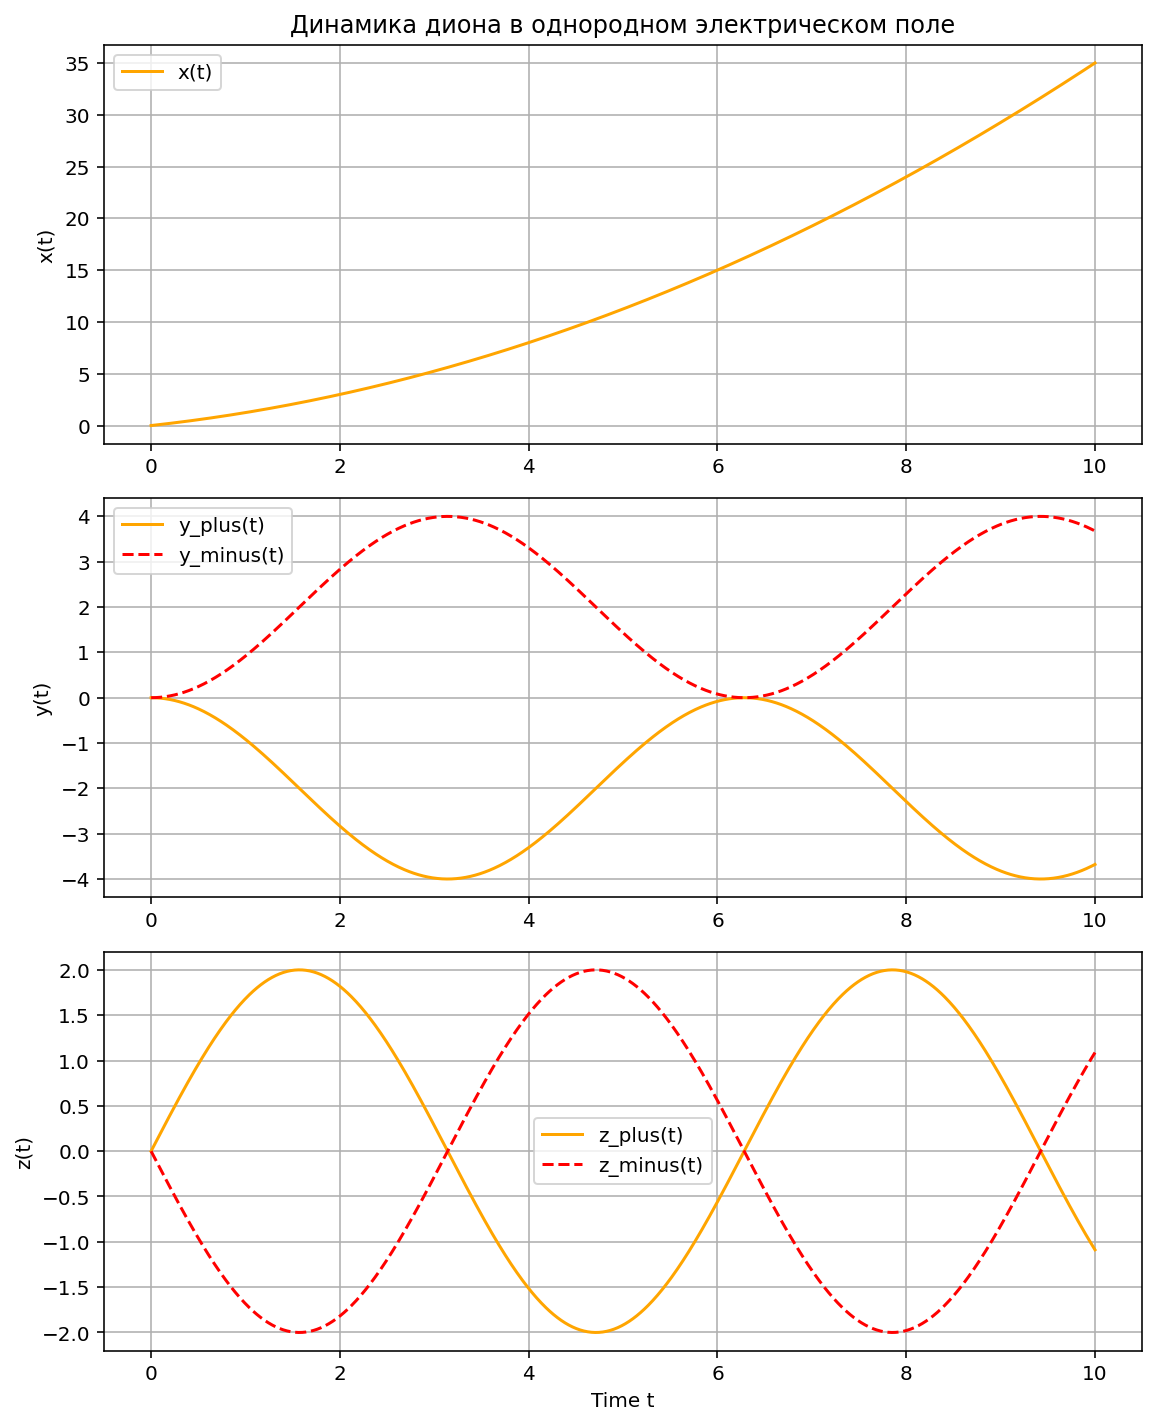
\includegraphics[width=0.65\textwidth]{dion_E.png}
		\label{fig:label}
		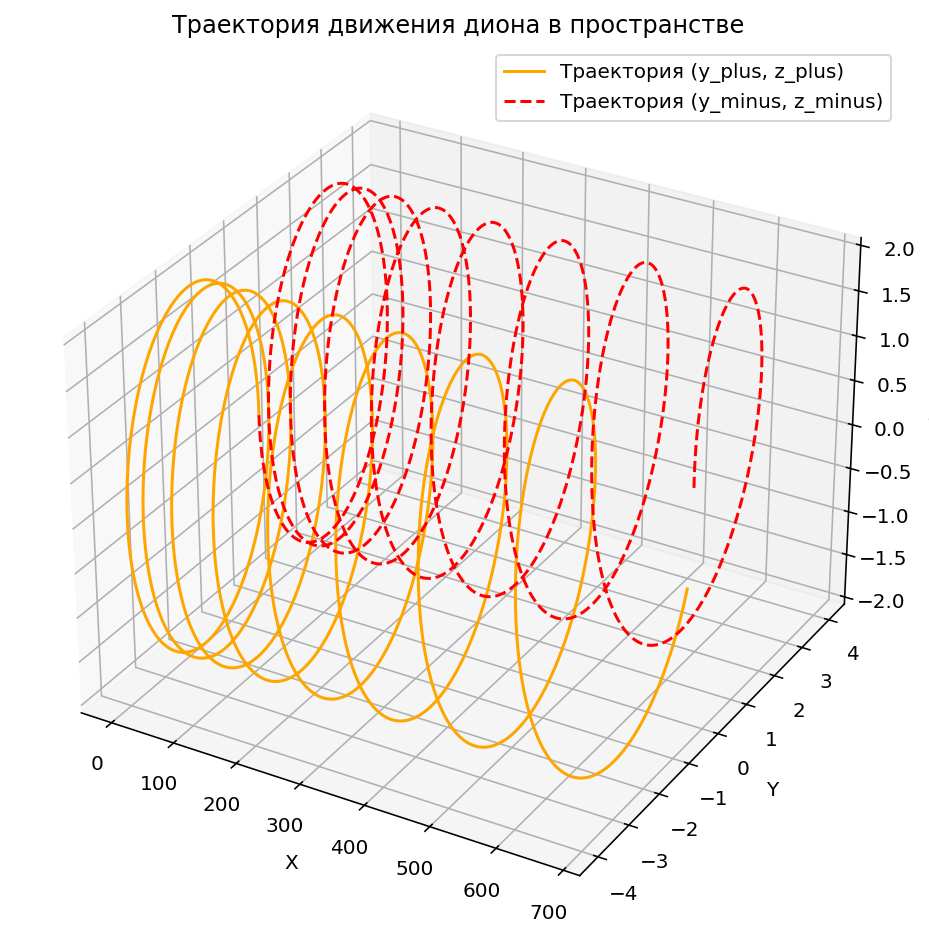
\includegraphics[width=0.65\textwidth]{dion_E_xyz.png}
		\label{fig:label_1}
	\end{figure}
	
	\newpage
	\subsubsection{Движение диона в однородном магнитном поле}
	
	\noindent Рассмотрим движение диона только в однородном магнитном поле $(\vec{B} = \vec{0})$, задающемся в пространстве вектором магнитном индукции вида $\vec{B} = \{0,\, B_{y},\, 0\}$. \\
	
	\noindent Запишем уравнение динамики для данного случая: \\
	
	\begin{math}
		\begin{aligned}
			& m\dot{\vec{v}} = B_{y}\Big(q_{\mu}\vec{e}_{y} + \frac{q_{e}}{c}\left(v_{x}\vec{e}_{z} - v_{z}\vec{e}_{x}\right)\Big)
		\end{aligned}
	\end{math} \\
	
	\noindent Рассмотрим следующую систему линейных дифференциальных уравнений $II$-го порядка относительно времени $t$: \\
	
	\begin{math}
		(\textasteriskcentered\textasteriskcentered) \left\{
		\begin{aligned}
			& \ddot{x} = -\frac{q_{e}B_{y}}{mc} \cdot \dot{z} \\\\
			& \ddot{y} =  \frac{q_{\mu}B_{y}}{m} \\\\
			& \ddot{z} = \frac{q_{e}B_{y}}{mc} \cdot \dot{x}
		\end{aligned}
		\right.
	\end{math} \\\\
	
	\noindent Произведём переобозначение вышеописанных групп констант: \\
	
	\begin{math}
		\begin{aligned}
			& \beta_{2} = \frac{q_{\mu}B_{y}}{m}, \quad \omega_{B} = \frac{q_{e}B_{y}}{mc}
		\end{aligned}
	\end{math} \\
	
	\noindent Перепишем систему уравнений $(\textasteriskcentered\textasteriskcentered)$ следующим образом: \\
	
	\begin{math}
		\left\{
		\begin{aligned}
			& \ddot{x} = -\omega_{B} \cdot \dot{z} \quad && (2.6) \\\\
			& \ddot{y} = \beta_{2} \quad && (2.7) \\\\
			& \ddot{z} = \omega_{E} \cdot \dot{x} \quad && (2.8)
		\end{aligned}
		\right.
	\end{math} \\
	
	\vskip1.5pt
	\noindent Данные уравнения приводят к аналогичному решению: \\
	
	\begin{math}
		\left\{
		\begin{aligned}
			& x = \pm \frac{v_{0_{x}}}{\omega_{B}} (\cos{\omega_{B}t} - 1) \\\\
			& y = \frac{\beta_{2}t^{2}}{2} + v_{0_{y}}t \\\\
			& z = \pm \frac{v_{0_{x}}}{\omega_{B}} \sin{\omega_{B}t}
		\end{aligned}
		\right.
	\end{math}
	
	\begin{figure}
		\centering
		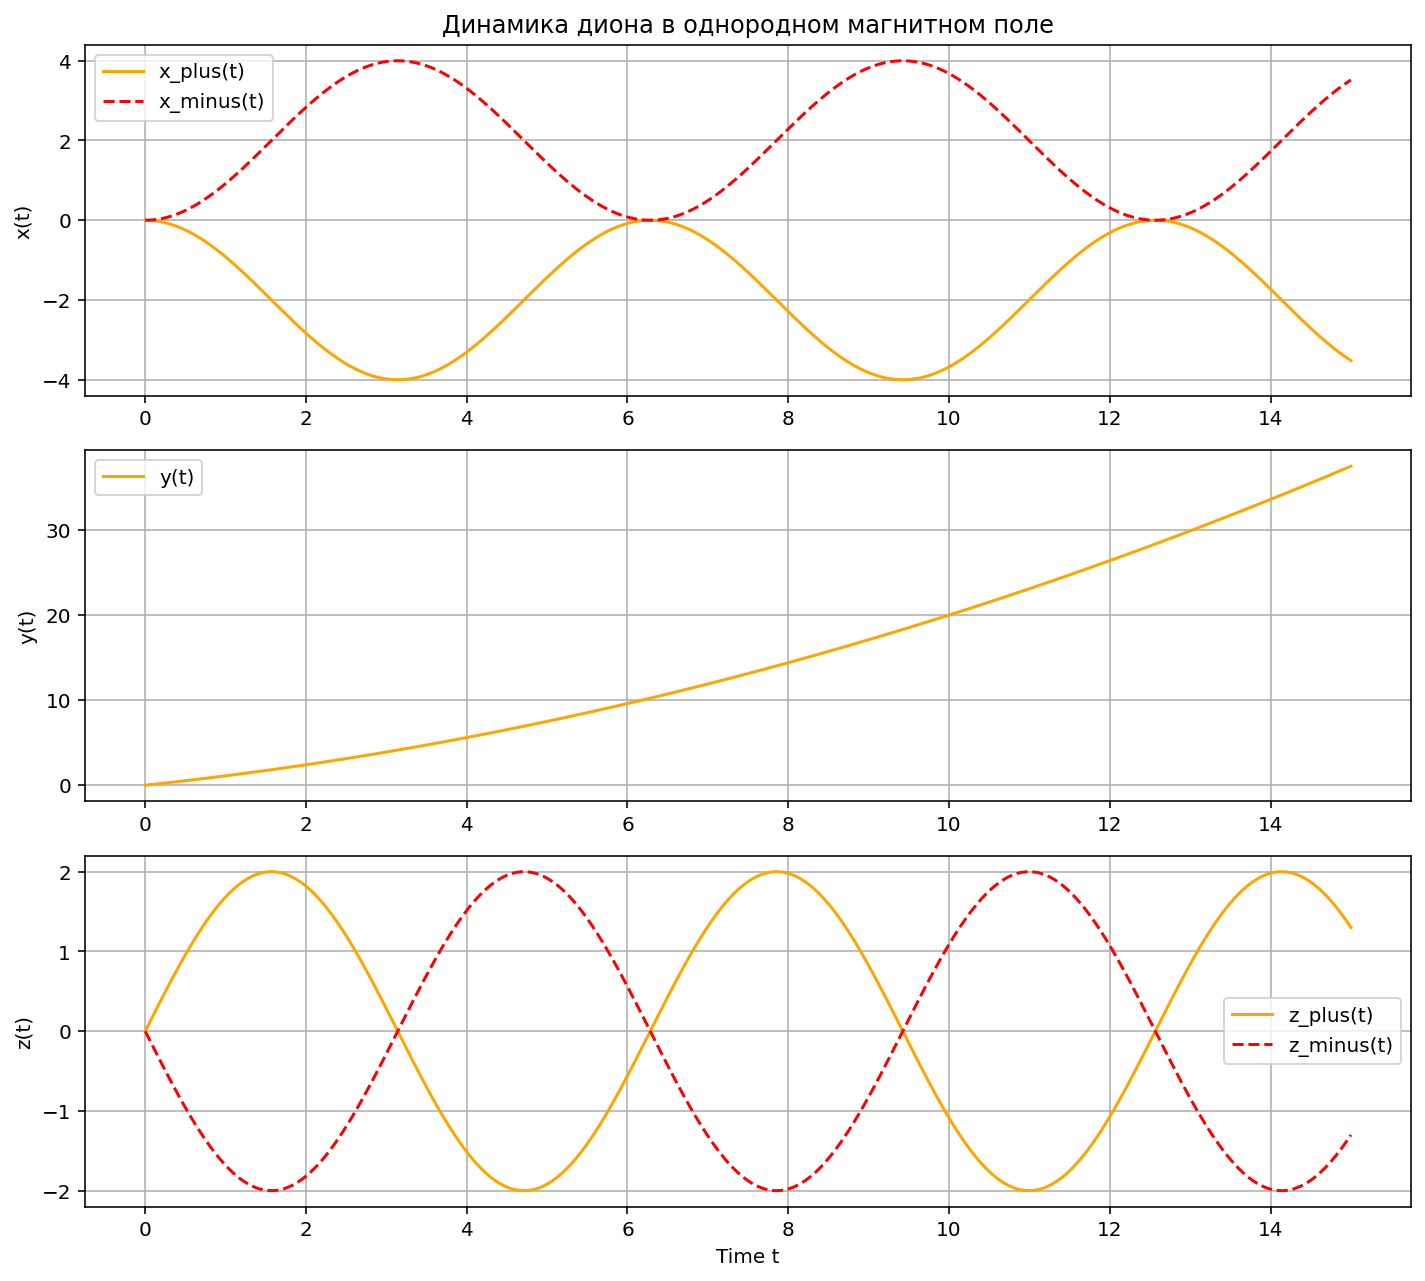
\includegraphics[width=0.7\textwidth]{dion_B.png}
		\label{fig:label1_1}
		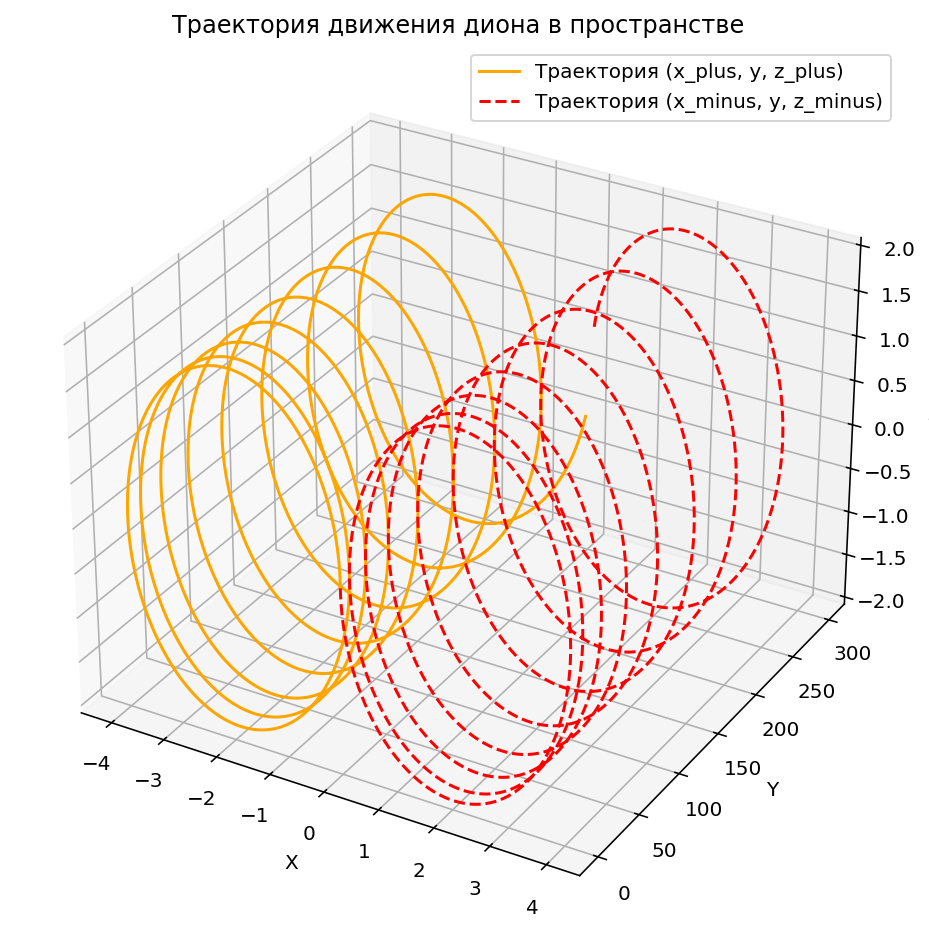
\includegraphics[width=0.7\textwidth]{dion_B_xyz.png}
		\label{fig:label_2}
	\end{figure}
	
	\newpage
	\subsubsection{Движение диона в скрещенных электрическом и магнитном полях}
	
	\noindent Рассмотрим движение диона в скрещенных однородных электрическом поле, задающемся в пространстве вектором электрической напряжённости вида $\vec{E} = \{E_{x},\, 0,\, 0\}$, и однородном магнитном поле, задающемся в пространстве вектором магнитной индукции индукции вида $\vec{B} = \{0,\, B_{y},\, 0\}$  \\
	
	\noindent Запишем уравнение динамики для данного случая: \\
	
	\begin{math}
		\begin{aligned}
			& m\dot{\vec{v}} = q_{e}\Big(E_{x}\vec{e}_{x} + \frac{1}{c}B_{y}\left(v_{x}\vec{e}_{z} - v_{z}\vec{e}_{x}\right)\Big) + q_{\mu}\Big(B_{y}\vec{e}_{y} - \frac{1}{c}E_{x}\left(v_{z}\vec{e}_{y} - v_{y}\vec{e}_{z}\right)\Big)
		\end{aligned}
	\end{math} \\
	
	\noindent Рассмотрим следующую систему линейных неоднородных дифференциальных уравнений $II$-го порядка относительно времени $t$: \\
	
	\begin{math}
		(\textasteriskcentered\textasteriskcentered\textasteriskcentered) \left\{
		\begin{aligned}
			& \ddot{x} + \frac{q_{e}B_{y}}{mc} \cdot \dot{z} = \frac{q_{e}E_{x}}{m} \\\\
			& \ddot{y} + \frac{q_{\mu}E_{x}}{mc} \cdot \dot{z} = \frac{q_{\mu}B_{y}}{m} \\\\
			& \ddot{z} = \frac{q_{e}B_{y}}{mc} \cdot \dot{x} + \frac{q_{\mu}E_{x}}{mc} \cdot \dot{y} 
		\end{aligned}
		\right.
	\end{math} \\\\
	
	\noindent Произведём переобозначение вышеописанных групп констант: \\
	
	\begin{math}
		\begin{aligned}
			& \beta_{1} = \frac{q_{e}E_{x}}{m}, \quad \omega_{E} = \frac{q_{\mu}E_{x}}{mc}, \quad \beta_{2} = \frac{q_{\mu}B_{y}}{m}, \quad \omega_{B} = \frac{q_{e}B_{y}}{mc}
		\end{aligned}
	\end{math} \\
	
	\noindent Перепишем систему уравнений $(\textasteriskcentered\textasteriskcentered\textasteriskcentered)$ следующим образом: \\
	
	\begin{math}
		\left\{
		\begin{aligned}
			& \ddot{x} + \omega_{B} \cdot \dot{z} = \beta_{1} \quad && (2.9) \\\\
			& \ddot{y} + \omega_{E} \cdot \dot{z} = \beta_{2} \quad && (2.10) \\\\
			& \ddot{z} = \omega_{B} \cdot \dot{x} + \omega_{E} \cdot \dot{y} \quad && (2.11)
		\end{aligned}
		\right.
	\end{math} \\\\
	
	\noindent При выражении из уравнения $(2.11)$ $\dot{x}$, подстановке его в уравнение $(2.9)$ и подстановке уравнения $(2.10)$ в получившееся уравнение, получим следующего вида линейное неоднородное дифференциальное уравнение $III$-го порядка относительно $t$: \\
	
	\begin{math}
		\begin{aligned}
			& \dddot{z} + (\omega_{E}^{2} + \omega_{B}^{2}) \cdot \dot{z} = \omega_{B}\beta_{1} + \omega_{E}\beta_{2} \quad && (2.12)
		\end{aligned}
	\end{math} \\
	
	\noindent Решая сие уравнение с учётом задачи Коши $(z(0) = 0,\ \dot{z}(0) = v_{0_{z}},\ \ddot{z}(0) = 0)$, получаем следующий вид функции $z(t)$: \\
	
	\begin{math}
		\begin{aligned}
			& z = \frac{B}{\Omega^{3}} \Big(\Omega t \pm \sin{\Omega t}\Big), \quad B = \omega_{B}\beta_{1} + \omega_{E}\beta_{2}, \quad \Omega = \sqrt{\omega_{B}^{2} + \omega_{E}^{2}} 
		\end{aligned}
	\end{math} \\\\
	
	\noindent Подставим получившееся уравнение $z = z(t)$ в уравнения $(2.9)$ и $(2.10)$ и найдём соответственно уравнения $x = x(t)$ и $y = y(t)$ c учётом аналогичной задачи Коши: \\
	
	\begin{math}
		\begin{aligned}
			& x = \bigg(\beta_{1} - \omega_{B} \cdot \frac{B}{\Omega^{2}}\bigg)\frac{t^{2}}{2} + v_{0_{x}}t \pm \omega_{B} \cdot \frac{B}{\Omega^{4}} \Big(\cos{\Omega t} - 1\Big) \\\\
			& y = \bigg(\beta_{2} - \omega_{E} \cdot \frac{B}{\Omega^{2}}\bigg)\frac{t^{2}}{2} + v_{0_{y}}t \pm \omega_{E} \cdot \frac{B}{\Omega^{4}} \Big(\cos{\Omega t} - 1\Big)
		\end{aligned}
	\end{math} \\\\
	
	\noindent В результате, получаем итоговую систему уравнений движения частицы: \\
	
	\begin{math}
		\left\{
		\begin{aligned}
			& x = \bigg(\beta_{1} - \omega_{B} \cdot \frac{B}{\Omega^{2}}\bigg)\frac{t^{2}}{2} + v_{0_{x}}t \pm \omega_{B} \cdot \frac{B}{\Omega^{4}} \Big(\cos{\Omega t} - 1\Big) \\\\
			& y = \bigg(\beta_{2} - \omega_{E} \cdot \frac{B}{\Omega^{2}}\bigg)\frac{t^{2}}{2} + v_{0_{y}}t \pm \omega_{E} \cdot \frac{B}{\Omega^{4}} \Big(\cos{\Omega t} - 1\Big) \\\\
			& z = \frac{B}{\Omega^{3}} \Big(\Omega t \pm \sin{\Omega t}\Big), \quad B = \omega_{B}\beta_{1} + \omega_{E}\beta_{2}, \quad \Omega = \sqrt{\omega_{B}^{2} + \omega_{E}^{2}}
		\end{aligned}
		\right.
	\end{math}
	
	\begin{figure}
		\centering
		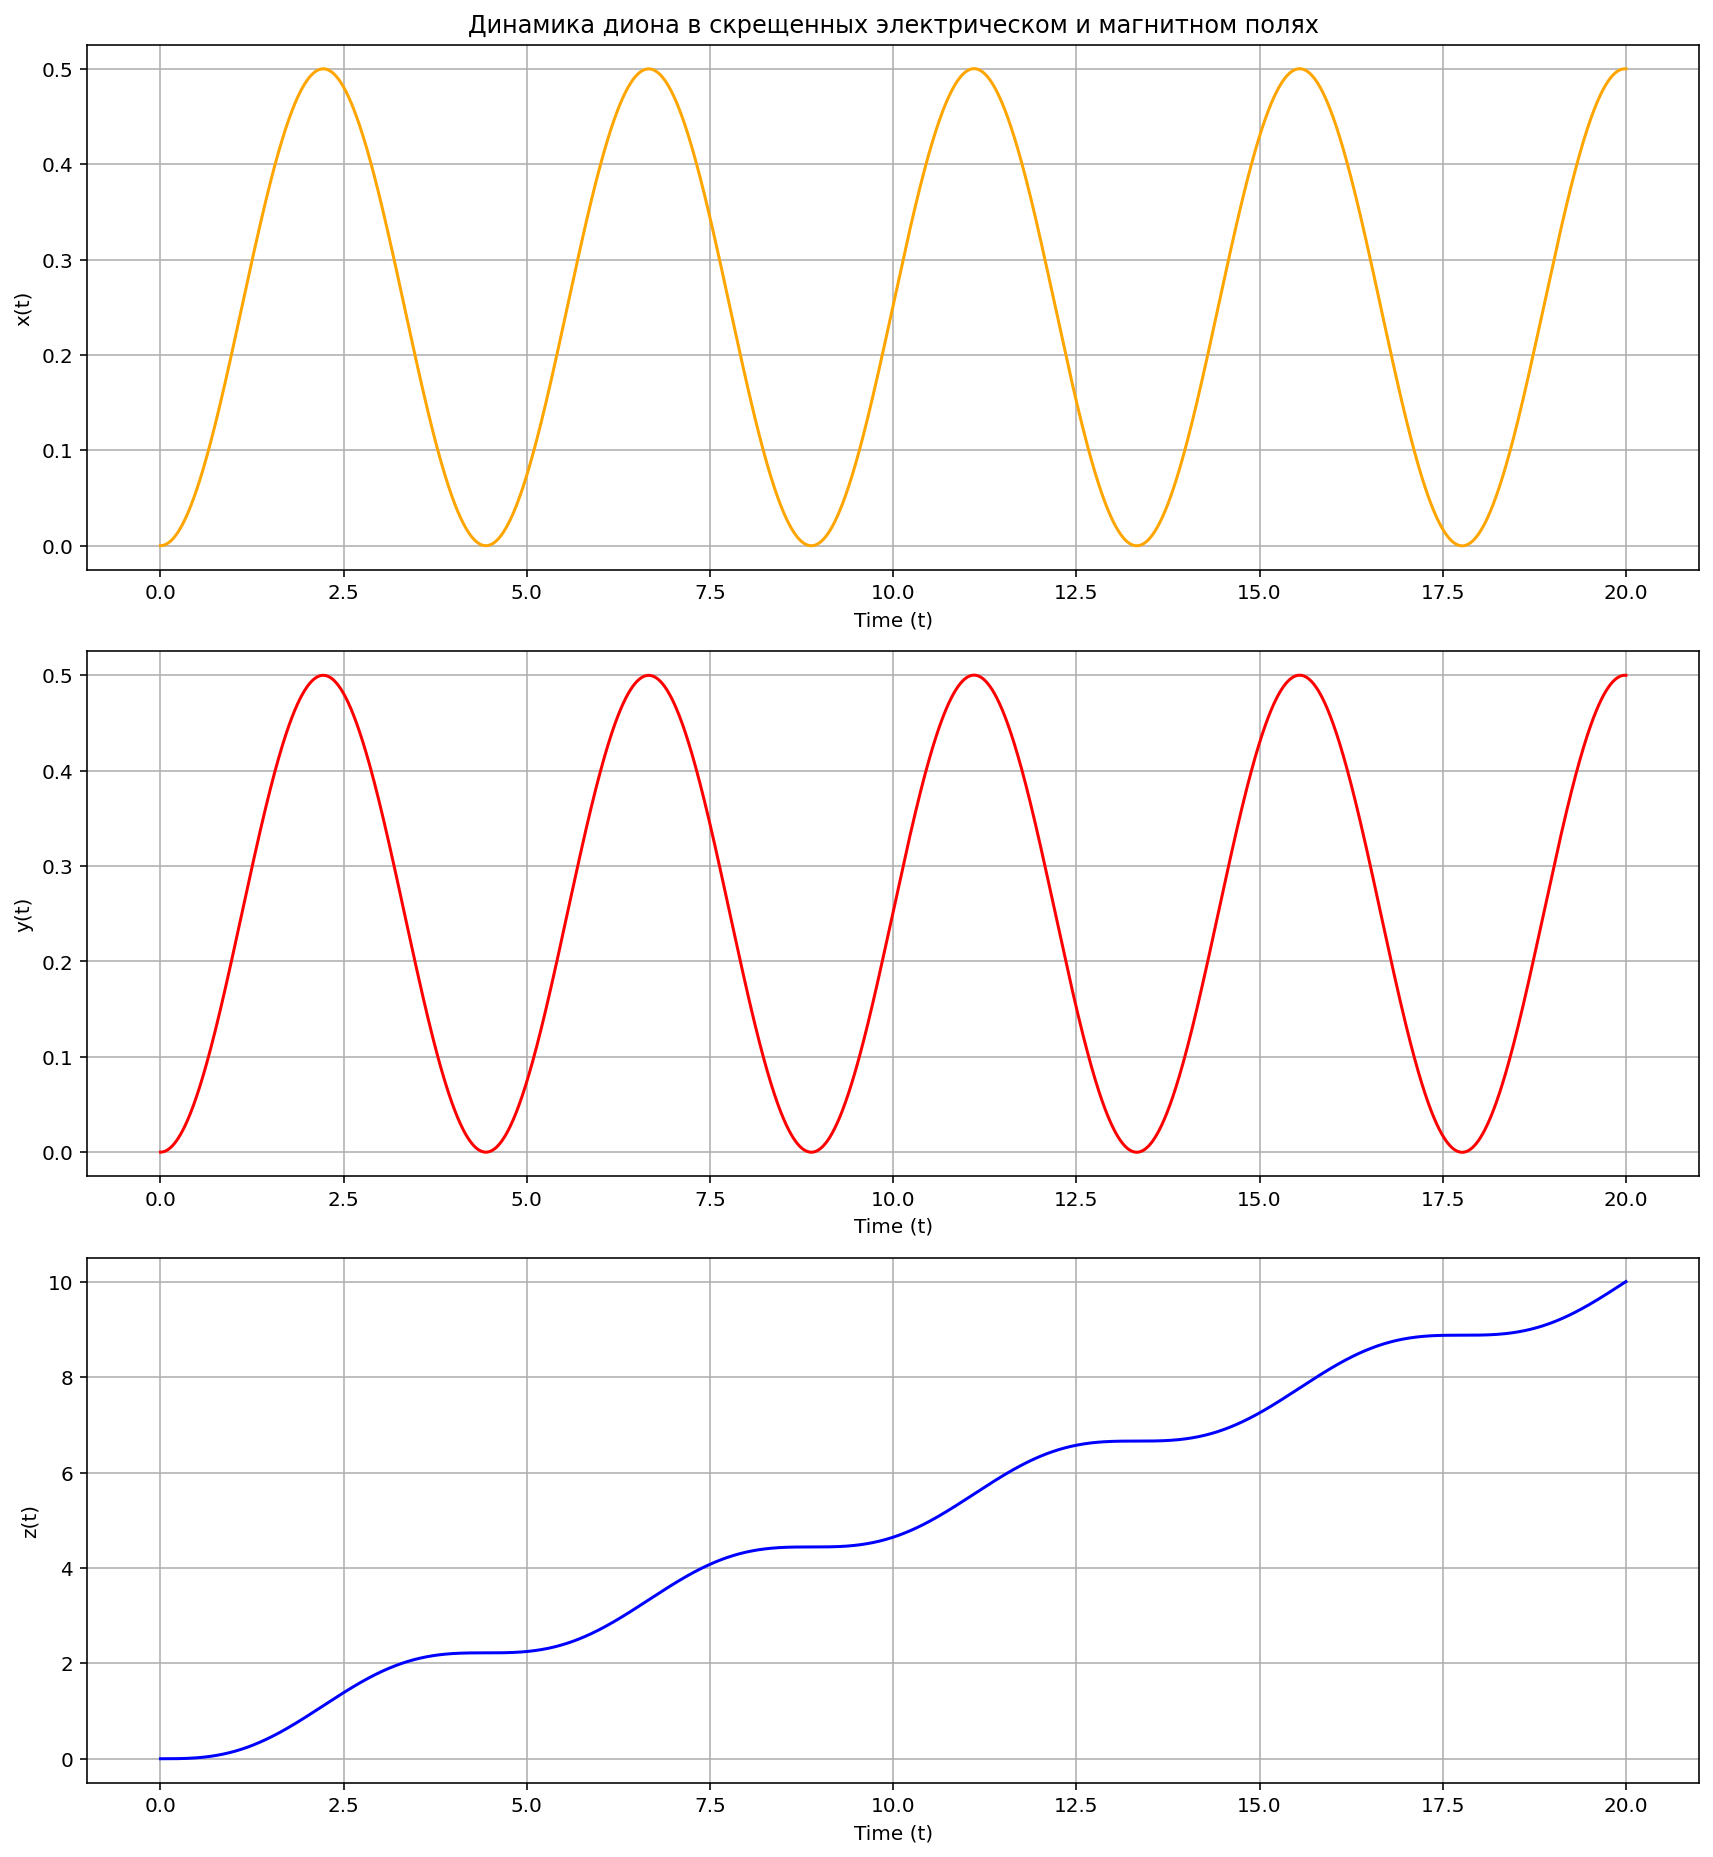
\includegraphics[width=0.65\textwidth]{dion_E_B.png}
		\label{fig:label_3}
		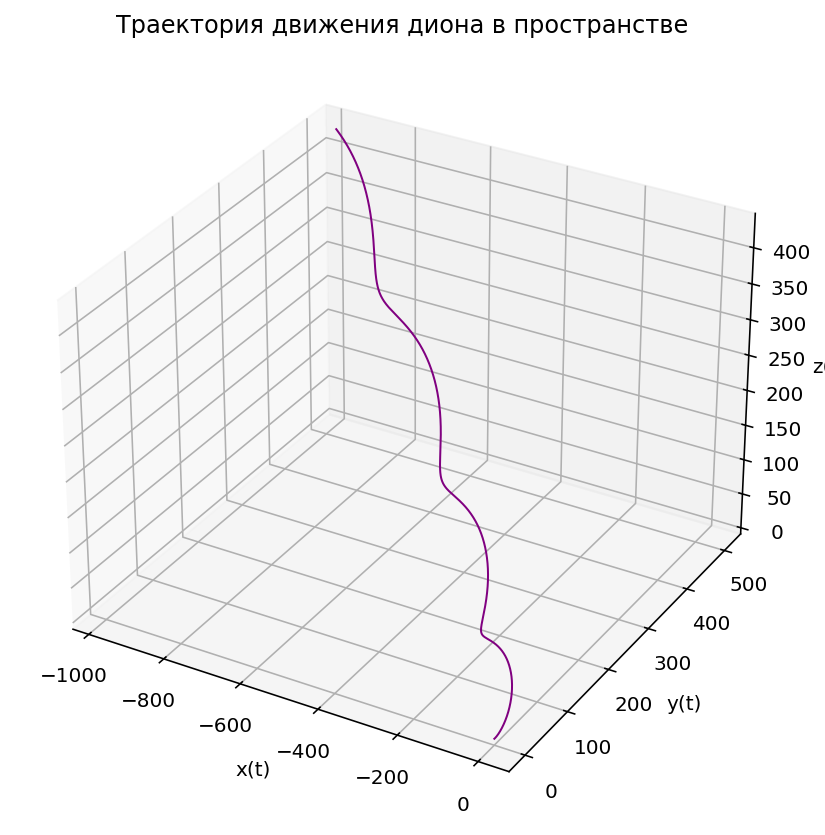
\includegraphics[width=0.65\textwidth]{dion_E_B_xyz.png}
		\label{fig:label_4}
	\end{figure}
	
	\begin{figure}
		\noindent На итоговом графике изображены траектории движения диона в трёх нами рассмотренных случаях: \\\\
		\centering
		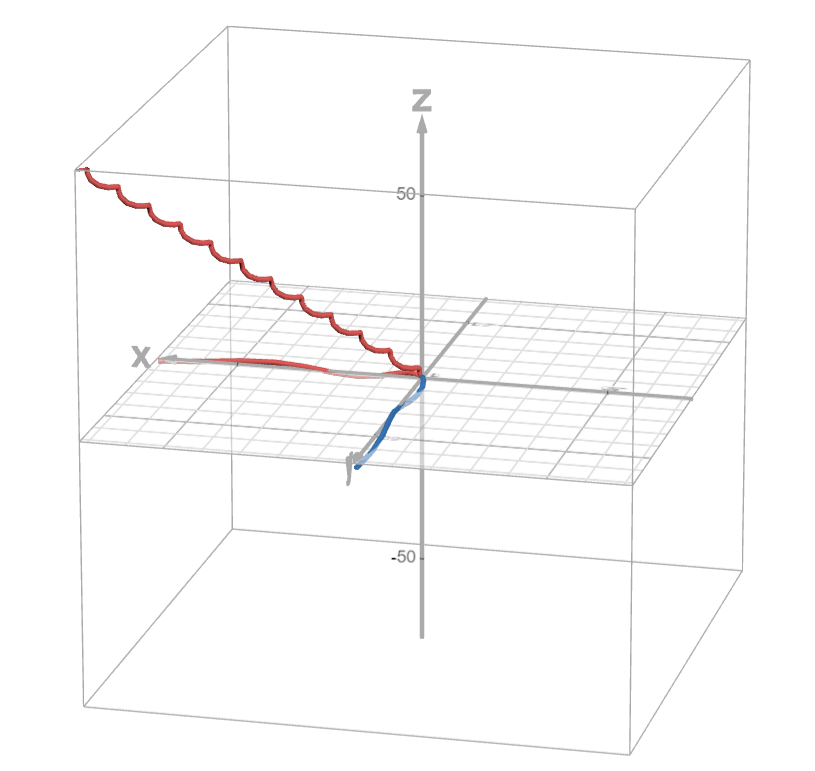
\includegraphics[width=0.65\textwidth]{all_trajectories.png}
		\label{fig:label_5}
	\end{figure}
	
	\vskip16pt
	\[
	\boxed{
		\begin{aligned}
			& \text{Интересно заметить, что при введении модели магнитного монополя} \\
			& \text{Дирака для описания элементарного магнитного заряда}\; q_{\mu} = \frac{\hbar c}{2q_{e}}, \\
			& \text{можно выразить постоянную тонкой структуры}\; \alpha = \frac{q_{e}}{2q_{\mu}}, \\
			& \text{определяющую силу электромагнитного взаимодействия,} \\
			& \text{следующим образом:}\; \alpha = \frac{\beta_{1}}{2 \omega_{E}c}
		\end{aligned}
	}
	\]
	\clearpage
	\section{Задача 2}
	\subsection{Аналитическое решение}
	\paragraph{Одномерная модель:}
	В рамках одномерной модели Изинга рассматривается цепочка из $N$ одинаковых магнитных моментов, которые могут быть ориентированы либо "вверх", либо "вниз". Считается, что взаимодействуют только соседние магнитные моменты, причем энергия их взаимодействия равна $-J$, если они направлены в одну сторону, и $J$, если в разные, где $J=const>0$ \textbf{---} квантовомеханическая энергия обменного взаимодействия. Также предполагается, что цепочка помещена в магнитное поле $\vec B$, и накладываются циклические граничные условия в виде взаимодействия первого и последнего атомов цепочки. Температура $T$ считается заданной изначально и постоянной. \\
	
	\noindent Формализуем всё перечисленное. Будем считать, что магнитные моменты заданы как $\vec \mu_{i}=\mu_{(1)}s_{i}\vec e_{z}$, где $\mu_{(1)}$\textbf{---} модуль магнитного момента, $s_{i} \in \{-1, 1\}$ \textbf{---} так называемый спин, и $\vec B=B\vec e_{z}$. В таком случае полная энергия цепочки записывается как 
	$$E=-J\sum_{i=1}^{N-1}s_{i}s_{i+1}-Js_{1}s_{N}-\mu_{(1)}B\sum_{i=1}^{N}s_{i}$$ \\
	
	\noindent В данной формуле первая сумма отвечает за энергию взаимодействия основной части цепочки, вторая сумма отвечает за энергию взаимодействия диполей и магнитного поля (которое предполагается классическим) и оставшееся слагаемое связано с циклическим граничным условием. \\
	
	\noindent Теперь будем искать статистическую сумму $Z$, через которую выразятся все интересующие нас величины (например, средняя намагниченность спинов). Как известно из экспериментов, в случае ферромагнетиков эти величины должны претерпевать скачок при некоторой температуре, называемой температурой Кюри $T_{c}$. \\
	
	\noindent Итак, статистическая сумма по конфигурациям цепочки $\{s\}$ запишется как
	$$Z=\sum_{\{s\}}e^{-\frac{E}{k_{B}T}}=\sum_{\{s\}}\exp\left(\frac{J}{k_{B}T}\sum_{i=1}^{N-1}s_{i}s_{i+1}+\frac{J}{k_{B}T}s_{1}s_{N}+\frac{\mu_{(1)}B}{k_{B}T}\sum_{i=1}^{N}s_{i}\right)$$
	Для удобства введём $\alpha=\frac{J}{k_{B}T}$ и $\beta=\frac{\mu_{(1)}B}{k_{B}T}$, после чего перепишем статистическую сумму в следующем виде:
	$$Z=\sum_{\{s\}}e^{\alpha s_{1}s_{2}+\frac{\beta}{2}(s_{1}+s_{2})}e^{\alpha s_{2}s_{3}+\frac{\beta}{2}(s_{2}+s_{3})}\ldots e^{\alpha s_{N}s_{1}+\frac{\beta}{2}(s_{N}+s_{1})}=\sum_{\{s\}}t_{s_{1}s_{2}}t_{s_{2}s_{3}}\ldots t_{s_{N}s_{1}}$$
	Где $t_{s_{i}s_{j}}=e^{\alpha s_{i}s_{j}+\frac{\beta}{2}(s_{i}+s_{j})}$. Оказывается, что из $t_{s_{i}s_{j}}$ можно сформировать так называемую трансфер-матрицу 
	$$T=
	\begin{pmatrix}
		T_{1, 1} & T_{1, -1} \\
		T_{-1, 1} & T_{-1, -1} \\
	\end{pmatrix}=
	\begin{pmatrix}
		e^{\alpha+\beta} & e^{-\alpha} \\
		e^{-\alpha} & e^{\alpha-\beta} \\
	\end{pmatrix}$$
	При этом будем обозначать элементы $T^{k}$ как $t^{(k)}_{1, 1}$, $t^{(k)}_{1, -1}$, $t^{(k)}_{-1, 1}$ и $t^{(k)}_{-1, -1}$.Тогда окажется, что 
	\begin{multline*}
		Z=\sum_{\{s\}}t_{s_{1}s_{2}}t_{s_{2}s_{3}}\ldots t_{s_{N}s_{1}}=\sum_{s_{1}=\pm 1}\sum_{s_{2}=\pm 1}\ldots\sum_{s_{N}=\pm 1}t_{s_{1}s_{2}}t_{s_{2}s_{3}}\ldots t_{s_{N}s_{1}}= \\= \sum_{s_{1}=\pm 1}\sum_{s_{2}=\pm 1}\ldots\sum_{s_{N-1}=\pm 1}t_{s_{1}s_{2}}t_{s_{2}s_{3}}\ldots t_{s_{N-2}s_{N-1}}\sum_{s_{N}=\pm 1}t_{s_{N-1}s_{N}}t_{s_{N}s_{1}}
	\end{multline*}
	Исходя из формул перемножения матриц получаем, что 
	$$\sum_{s_{N}=\pm 1}t_{s_{N-1}s_{N}}t_{s_{N}s_{1}}=t^{(2)}_{s_{N-1}s_{1}}$$
	Повторяя подобные перестановки сумм и преобразования произведений получим, что 
	$$Z=\sum_{s_{1}=\pm 1}t^{(N)}_{s_{1}s_{1}}=Tr \ T^{N}$$
	В нашем случае, матрица $T$ очевидно является симметричной и обладает вещественными элементами, что позволяет привести её к диагональному виду 
	$$
	T^\prime=
	\begin{pmatrix}
		\lambda_{1} & 0 \\
		0 & \lambda_{2} \\
	\end{pmatrix}
	$$
	Причем из-за инвариантности следа матрицы окажется, что 
	$$Z=Tr \ T^{N}=Tr \ T^{\prime N}=\lambda_{1}^N+\lambda_{2}^{N}$$
	Если процедуру диагонализации провести так, чтобы $\lambda_{1} > \lambda_{2}$ (собственные значения обязательно будут вещественными из-за того, как была определена матрица), то в предельном случае $N\rightarrow \infty$ получим 
	$$Z=\lambda_1^{N}$$
	Для нашего определения матрциы $T$ имеем характеристическое уравнение 
	$$\lambda^2-\lambda(e^{\alpha+\beta}+e^{\alpha-\beta})+e^{2\alpha}-e^{-2\alpha}=0$$
	Отсюда получаем, что 
	$$\lambda_{\pm}=e^{\alpha}\cosh(\beta)\pm\sqrt{e^{2\alpha}\sinh^{2}(\beta)+e^{-2\alpha}}$$
	И тогда $\lambda_{1}=e^{\alpha}\cosh(\beta)+\sqrt{e^{2\alpha}\sinh^{2}(\beta)+e^{-2\alpha}}$, откуда свободная энергия приходящаяся на один спин равна $F=-\frac{k_{B}T}{N}\ln Z=-k_{B}T\left(\alpha+\ln\left(\cosh(\beta)+\sqrt{\sinh^{2}(\beta)+e^{-4\alpha}}\right)\right)$. Если также считать, что каждый спин занимает объём $V$, то средняя намагниченность будет равна 
	$$\langle M \rangle=-\frac{1}{V}\frac{\partial f}{\partial B}=-\frac{\mu_{(1)}}{Vk_{B}T}\frac{\partial f}{\partial \beta}=M_{(1)}\frac{\sinh(\beta)}{\sqrt{\sinh^2(\beta)+e^{-4\alpha}}}$$
	Или, подставив значения $\alpha$ и $\beta$, получим ответ на вопрос задачи для одномерной цепочки:
	$$\boxed{\langle M \rangle = M_{(1)}\frac{\sinh\left(\frac{\mu_{(1)}B}{k_{B}T}\right)}{\sqrt{\sinh^2\left(\frac{\mu_{(1)}B}{k_{B}T}\right)+e^{-\frac{4J}{k_{B}T}}}}}$$ \\
	
	\noindent При $B\rightarrow 0$ имеем $\langle M \rangle=M_{(1)}e^{-\frac{4J}{k_{B}T}}\frac{\mu_{(1)}B}{k_{B}T} \Rightarrow \langle M \rangle \sim B$, что соответствует парамагнетику, а не ферромагнетику. Также из полученной формулы видно, что при $T>0$ намагниченность не терпит разрывов, что тоже не согласуется с известными свойствами ферромагнетиков. \\ 
	
	\noindent Если проанализировать иные параметры системы (например, удельную теплоемкость, которая скачком изменяется при фазовом переходе второго рода), то мы также не обнаружим ожидаемых разрывов. Таким образом, одномерная модель Изинга не описывает реальность в полной мере.
	
	\newpage 
	\paragraph{Двумерная и трехмерная модели:}
	Точное аналитическое решение для двумерной модели Изинга вполне возможно, однако его получение и анализ крайне трудны с точки зрения математики, так что здесь мы ограничимся кратким изложением основных этапов его получения и важными в дальнейшем результатами. Полное изложение можно прочитать, например, в \S 151 \cite{land5}. \\
	
	\noindent В рамках этого решения для двумерной модели рассматривается плоская квадратная решетка из $N$ узлов при отсутствии магнитного поля. Аналогично одномерному случаю, записывается полная энергия системы диполей, после чего записывается статистическая сумма. Полученная экспонента раскладывается по степеням $\theta = \frac{J}{k_{B}T}$, в результате чего статистическая сумма представляется в виде полинома по степеням $x=\tanh(\theta)$ и по степеням спинов. После этого каждому одночлену ставится в соответствие некоторый цикл на решетке (который может иметь самопересечения и быть многосвязным). Каждый цикл представляется в виде совокупности нескольких замкнутых петель, по которым проводится суммирование. Оно, в свою очередь, сводится к уже решенной задаче о случайных блужданиях точки по решетке. После длительных математическх преобразований находится статистическая сумма в виде двойного произведения и термодинамический потенциал в виде интеграла, не берущегося в элементарных функциях. \\
	
	\noindent Дальнейший анализ и получение критических показателей оказывается ещё сложнее, так что опишем наиболее интересные его результаты. Во-первых, двумерная модель (в отличие от одномерной) не теряет интересующие нас свойства ферромагнетиков, что позволяет попробовать её использовать для описания реальных объектов. Во-вторых, в рамках данной модели получается, что температура Кюри равна $T_{c}=\frac{2J}{k_{B}\ln(1+\sqrt{2})}$. В дальнейшем эта формула позволит оценить значение параметра $J$ для проведения компьютерного моделирования. \\
	
	\noindent В свою очередь, аналитическое решение трехмерной модели на данный момент отсутствует, и непонятно, насколько реально его получение.
	
	\newpage
	\subsection{Компьютерное моделирование:}
	\paragraph{Одномерная и трехмерная модели:}
	Компьютерное моделирование одномерной модели не проводилось в связи с тем, что возможно её точное аналитическое решение, из которого следует, что одномерная модель теряет часть важных свойств ферромагнетика. \\
	
	\noindent В свою очередь, моделирование трехмерной задачи не проводилось в связи с тем, что имеющееся оборудование и реализации алгоритма не позволяют проводить моделирование достаточно больших систем с достаточной скоростью. Однако это принципиально возможно при наличии более мощных компьютеров и лучшей оптимизации соответствующих алгоритмов.
	
	\paragraph{Двумерная модель:}
	Рассмотрим сперва постановку задачи для двумерной модели. Аналогично одномерной модели определяются магнитное поле $\vec B$, энергия обменного взаимодействия $J$, а также  магнитные моменты $\vec \mu_{i,\ j}$ и спины $s_{i,\ j}$, которые сейчас имеют два индекса, причем $i=\overline{1, N_{x}}$ и $j=\overline{1, N_{y}}$ \textbf{---} в модели рассматривается прямоугольная сетка спинов. Также налагаются циклические граничные условия: спины $s_{0,\ j}$ взаимодействуют со спинами $s_{N_{x}, \ j}$, а спины $s_{i, \ 0}$ \textbf{---} со спинами $s_{i, \ N_{y}}$. Тогда энергия такой решетки запишется как 
	$$E=-J\sum_{i = 0}^{N_{x}}\sum_{j=0}^{N_{y}}s_{i, \ j}S_{i, \ j}-\mu_{(1)}B\sum_{i = 0}^{N_{x}}\sum_{j=0}^{N_{y}}s_{i, \ j}$$
	где $S_{i, \ j}$ \textbf{---} сумма спинов, соседних с $s_{i, \ j}$ с учетом граничных условий. \\
	
	\noindent Для проведения моделирования будем использовать метод Монте-Карло для канонического ансамбля. Опишем его в приложении к нашей задаче. В ходе одного шага этого метода выполняются следующая последовательность действий:
	\begin{enumerate}
		\item Выбирается случайный спин $s_{i, \ j}$.
		\item Подсчитывается возможное изменение энергии системы $\Delta E$ при его перевороте. 
		\item Генерируется равномерно распределенное на отрезке $[0; \ 1]$ случайное число $r$.
		\item Если $\Delta E < 0$ или если $r<e^{-\frac{\Delta E}{k_{B}T}}$, то переворот спина принимается.
		\item Если переворот спина принимается, то обновляются и сохраняются новые значения энергии $E$ и полного магнитного момента $\mu_{\Sigma}$ системы. Иначе сохраняются их предыдущие значения.
	\end{enumerate}
	
	\noindent Далее, в ходе одной итерации метода Монте-Карло проводится $N_{x} \cdot N_{y}$ таких шагов. В свою очередь, количество итераций зависит от интересующего нас расчета. При инициализации расчета, ориентация спинов на сетке генерируется случайно, после чего подсчитывается $E$ и $\mu_{\Sigma}$. \\
	
	\noindent Данный алгоритм был реализован в среде Matlab с применением различных оптимизаций, таких как векторизация, предварительная генерация случайных чисел, предварительный подсчет возможных $\Delta E$ (оказывается, что множество этих значений достаточно ограничено) и иных. Это, в свою очередь, позволилило проводить все симуляции при $N_{x}=N_{y}=100$ за приемлимое время при достаточно большом общем количестве итераций. \\
	
	\noindent Проводилось два основных типа симуляций, которые сильно отличаются друг от друга.
	\begin{itemize}
		\item В ходе симуляций первого типа были получены кривые гистерезиса. Для этого задавалось переменное магнитное поле $B=B_{max}\sin(\omega t)$, и за каждый шаг времени $\Delta t$ проводилась одна итерация метода. На вход итерации подавалась сетка спинов, полученная в конце предыдущей итерации. В итоге сохранялись значения $B(t)$ и $\mu_{\Sigma}(t)$ в конце итераций, после чего проводилось усреднение по всем полным циклам, прошедшим за время симуляции и рассчитываласm намагниченность в каждый момент времени $M(t)=\frac{\mu_{\Sigma}(t)}{N_{x}N_{y}V}$
		\item В ходе симуляций второго типа были сделаны попытки получить графики намагниченности и удельной теплоемкости от температуры при нулевом магнитном поле. Для этого при каждом значении температуры от $T_{min}$ до $T_{max}$ с шагом $\Delta T$ проводились симуляции из 10000 итераций, по результатам которых рассчитывались $\langle M \rangle =\frac{\langle \mu_{\Sigma} \rangle}{N_{x}N_{y}V}$ и $c_{V}=\frac{1}{k_{B}T^2}\frac{1}{N_{x}N_{y}\rho V}(\langle E^2 \rangle - {\langle E \rangle}^2)$
	\end{itemize}
	
	\begin{figure}[h]
		\centering
		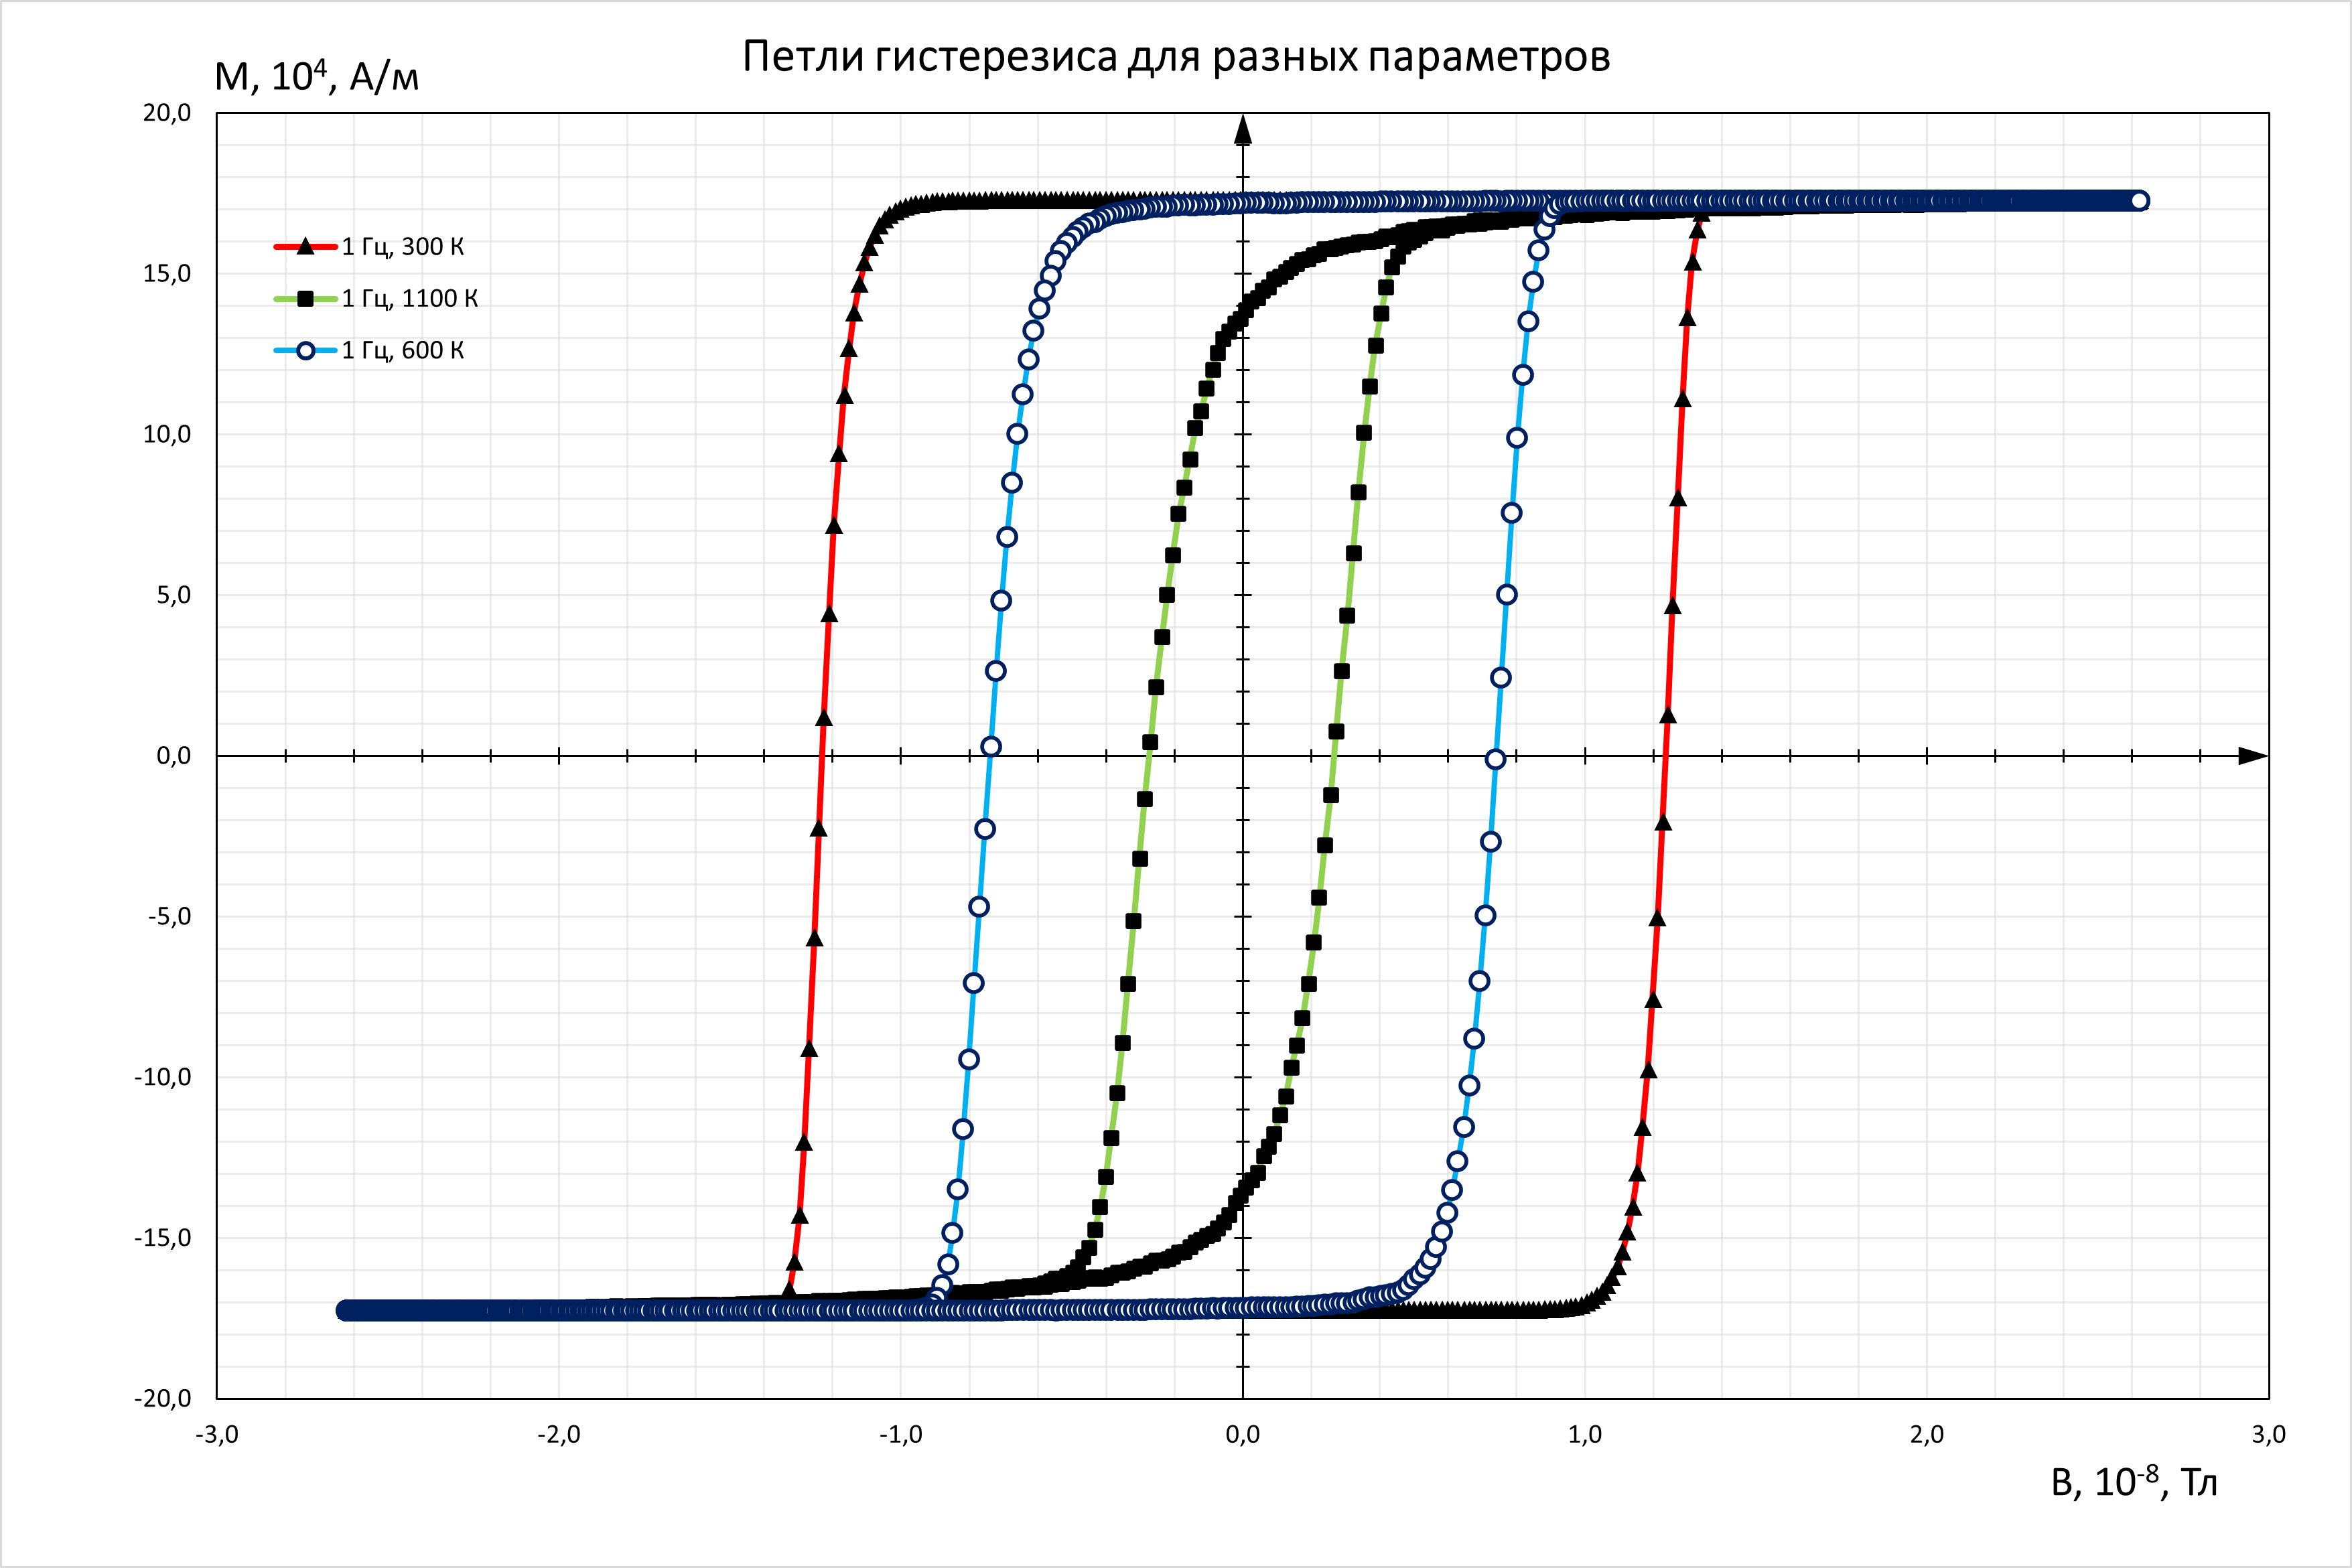
\includegraphics[scale=0.6]{fig1orig.png}
		\caption{График петель гистерезиса при частоте $\nu=\frac{\omega}{2\pi}=1 \ \text{Гц}$ и разных температурах $T$}
		\label{ris:hyst1}
	\end{figure}
	\begin{figure}[h]
		\centering
		\subfloat[\centering $T=300 \ \text{К}$] {{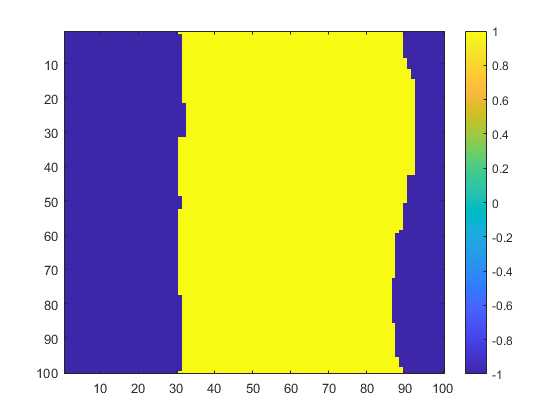
\includegraphics[scale=0.5]{fig2orig.png}}}
		\qquad
		\subfloat[\centering $T=1200 \ \text{К}$] {{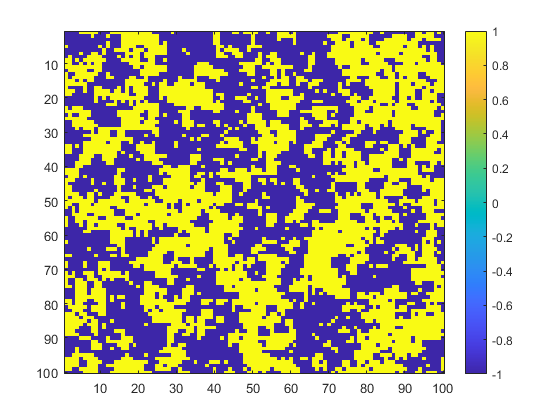
\includegraphics[scale=0.5]{fig3orig.png}}}
		\caption{Ориентация спинов при различных температурах. Упорядоченная и неупорядоченная структуры.}
		\label{ris:orient}
	\end{figure}
	
	\noindent Обсудим полученные результаты:
	\begin{itemize}
		\item Получены графики петель гистерезиса для нескольких наборов параметров и инструмент для их построения.
		\item Из рис. \ref{ris:hyst1} видно, что с повышением температуры петли гистерезиса меняют форму и сужаются. 
		\item При этом, в модели присутствует вычислительный артефакт: "ширина" петли гистерезиса зависит от отношения периода колебаний поля к шагу по времени. Для построения рис. \ref{ris:hyst1} использовалось $\frac{T}{\Delta t}=1000$, однако насколько это значение соответствует реальности \textbf{---} неизвестно. Возможно, правильное отношение можно найти с помощью экспериментов над реальными образцами или из соображений динамики фазовых переходов. К сожалению, таких возможностей у авторов сейчас нет. 
		\item Получить графики намагниченности и удельной теплоемкости, наглядно показывающие скачок вблизи температуры Кюри не получилось. При этом полученные значения удельной теплоемкости никак не соответствуют реальности: часть значений получалась отрицательной, а положительные значения оказывались примерно на 10 порядков меньше, чем табличные для железа. Полученный результат объясняется, скорее всего, ошибочным решением изучать модель ``с размерностями'', а также некорректной моделью для определения $J$, $\mu_{(1)}$ и $V$. В результате даже при большом числе итераций разброс значений получается крайне большой.
		\item Получены примеры (см. рис \ref{ris:orient} ниже) ориентации спинов при температурах больше, и меньше температуры Кюри, которые соответствуют теории. 
	\end{itemize}
	
	\newpage
	\paragraph{Получение исходных данных для моделирования:}	
	В рамках компьютерного моделирования можно анализировать как обезразмеренные модели, так и модели с реальными параметрами. Именно второй случай реализован в данной работе. \\
	
	\noindent Для того, чтобы промоделировать двумерную модель Изинга необходимо оценить $J$, $\mu_{1}$ и $V$. Будем работать в системе СИ и оценивать данные параметры для железа. Опиратся будем на вышеупомянутую формулу для температуры Кюри и на книгу \cite{magn}, из которой взяты часть параметров железа и формулы для оценки размера домена. \\
	
	\noindent Использовались следующие параметры железа: 
	\begin{itemize}
		\item Температура Кюри: $T_c=1043 \ \text{К}$
		\item Магнитный момент одного атома железа: $\mu_{Fe}=2.22\mu_{B}$ \footnote{$\mu_{B}$ \textbf{---} магнетон Бора}
		\item Кристаллическая решетка: объёмноцентрированная кубическая (ОЦК)
		\item Параметр решетки: $a=2.856 \cdot 10^{-10} \ \text{м}$
		\item Константа кубической анизотропии: $K=4.8 \cdot 10^{4} \ \frac{\text{Дж}}{\text{м}^3}$
		\item Молярная масса: $m_{mol, \ Fe}=0.056 \ \frac{\text{кг}}{\text{моль}}$
		\item Плотность: $\rho_{Fe}=7800 \ \frac{\text{кг}}{\text{м}^3}$
	\end{itemize}
	
	\noindent Как было упомянуто в разделе об аналитическом решении для двумерной модели Изинга, $T_{c}=\frac{2J}{k_{B}\ln(1+\sqrt{2})} \Rightarrow J=\frac{k_{B}T_{c}\ln(1+\sqrt{2})}{2} \Rightarrow \boxed{J \approx 6.343 \cdot 10^{-21} \ \text{Дж}}$. \\
	
	\noindent Как известно, ферромагнетики имеют доменную структуру. Будем считать, что каждый спин в симуляции соответствует одному реальному домену, каждый из которых имеет форму шара с радиусом $r_{c}$, который является критическим для домена при данных условиях (то есть при дальнейшем увеличении размера, энергетически более выгодной оказывается конфигурация, в которой большой домен разбит на два меньших). Также считается, что домены всегда ориентированны параллельно оси $OZ$. В книге \cite{magn} в разделе 6.7 показывается, что при таких условиях $r_{c}=\frac{9\sigma_{W}}{\mu_{0}M_{Fe}^2}$, если $r_{c}\gg \delta_{W}$. В данных формулах $\sigma_{w}$ \textbf{---} удельная энергия доменной стенки, $\delta_{w}$ \textbf{---} толщина доменной стенки и $M_{Fe}$ \textbf{---} намагниченность материала домена. \\
	
	\noindent Будем предполагать, что в домене магнитные моменты всех атомов направлены в одну сторону. Тогда исходя из определения намагниченности как магнитного момента единицы объёма вещества имеем $M=\frac{\mu_{Fe}N_{Fe}}{\Delta V}=\frac{\mu_{Fe}m_{Fe}N_{a}}{m_{mol, \ Fe}\Delta V}=\frac{\mu_{Fe}\rho_{Fe}N_{a}}{m_{mol, \ Fe}}\approx 1.727 \cdot 10^{5} \ \frac{\text{А}}{\text{м}}$. \\
	
	\noindent Для ОЦК имеем $\delta_{w}=\pi \sqrt{\frac{2JJ}{Ka}}\approx 9.557\cdot 10^{-8} \ \text{м}$ и $\sigma_{w}=\pi \sqrt{\frac{2JK}{a}}\approx 0.0046 \ \frac{\text{Дж}}{\text{м}^2}$\footnote{Строго говоря, вычисленное нами ранее значение $J$ характеризует обменное взаимодействие между доменами, тогда как тут оно характеризует взаимодействие между атомами, и потому отличается. Однако во-первых, у авторов нет иного хорошего способа оценить $J$, а во-вторых, можно надеяться, что эти значения совпадают по порядку, например из-за того, что в отсутствии магнитного поля модель Изинга для атомов и для доменов должны иметь одинаковые температуры Кюри.}. Тогда $r_{c} \approx 1.102 \cdot 10^{-6} \ \text{м}$, откуда $V=\frac{4}{3}\pi r_{c}^3 \Rightarrow \boxed{V \approx 5.609 \cdot 10^{-18} \ \text{м}^3}$ и $\mu_{(1)}=VM_{Fe} \Rightarrow \boxed{\mu_{(1)}\approx 9.687 \cdot 10^{-13} \text{А}\cdot\text{м}^2}$ \\
	
	\noindent Погрешности данных величин не оценивались.
	
	\newpage
	\section{Задача 3}
	
	\noindent Сперва сузим постановку задачи. Рассмотрение движения одиночной частицы (особенно \textbf{---} движения релятивистского) в плазме сопряжено с большими трудностями и требует скорее специфического численного моделирования. Поэтому было выбрано следующее сужение задачи: исследовать потенциал, электрическое поле и распределение зарядов в плазме при равномерном движении пробной частицы.В первую очередь будем рассматривать релятивистский случай, работать будем в системе СГС. \\ 
	
	\noindent Пусть $\vec R=\vec r - \vec r_{0}$, где $\vec r$ \textbf{---} радиус-вектор наблюдателя, $\vec r_{0}$ \textbf{---} радиус-вектор пробной частицы с зарядом $Q$. Тогда $\vec V = \dot {\vec R}=-\vec v_{0}$ и $\vec \beta = \frac{\vec V}{c}=-\frac{\vec v_{0}}{c}=-\vec \beta_{0}$ \textbf{---} безразмерная скорость. Тажке пусть $\lambda_D$ \textbf{---} дебаевский радиус плазмы, в которой движется частица.
	
	\begin{center}
		\begin{tikzpicture}[scale=2]
			% Draw axes with ultra thick lines
			\draw[->, thick] (0,0,0) -- (3,0,0) node[anchor=north east] {$y$};
			\draw[->, thick] (0,0,0) -- (0,3,0) node[anchor=north west] {$z$};
			\draw[->, thick] (0,0,0) -- (0,0,3) node[anchor=south] {$x$};
			
			% Label origin
			\node at (0,0,0) [below right] {$O$};
			
			% Add vectors and annotations with ultra thick lines
			\draw[->, thick, blue] (0,0,0) -- (3,1,1) node[midway, anchor=south west] {$\vec{r}$};
			\draw[->, thick, red] (0,0,0) -- (1.5,2,1) node[midway, anchor=south east] {$\vec{r}_0$};
			\draw[->, thick, green] (1.5,2,1) -- (3,1,1) node[midway, anchor=south] {$\vec{R}$};
		\end{tikzpicture}
	\end{center}
	
	\noindent Тогда рассмотрим систему координат, в которой пробная частица покоится (будем обозначать эту СО штрихом). В ней, согласно курсу физики плазмы (например, \cite{plasma}) потенциал экранированного заряда равен 
	
	$$\varphi^{\prime} = \frac{Q}{R^{\prime}}\exp\left(-\frac{R^{\prime}}{\lambda_D}\right)$$ \\
	
	\noindent Отсюда, из определения потенциала и уравнений Максвелла получаем
	
	$$\vec E^{\prime} = -\nabla \varphi^{\prime} = \frac{Q}{R^{\prime 2}}\exp\left(-\frac{R^{\prime}}{\lambda_{D}}\right)\left(\frac{1}{R^{\prime}}+\frac{1}{\lambda_D}\right)\vec R^{\prime}$$
	$$\rho^{\prime}=\nabla \cdot {\vec E^{\prime}}=-\frac{Q}{4\pi\lambda_D^2 R^{\prime}}\exp\left(-\frac{R^{\prime}}{\lambda_D}\right)$$ \\
	
	\noindent Следуя статье \cite{li-wich}, повторим для этих величин те операции, которые проводятся при выводе потенциалов и полей Лиенара-Вихерта:
	$$\gamma=\frac{1}{\sqrt{1-\beta^2}}, \ \varphi=\gamma\varphi^{\prime}, \ \vec E_{\perp}=\gamma\vec E^{\prime}_{\perp}, \ \vec E_{\|}=\vec E^{\prime}_{\|}, \ \rho=\gamma\rho^{\prime}$$
	$$t_{ret}=\frac{R}{c}, \ \vec R^{\prime}_{\perp}=\vec R_{\perp}, \ \vec R^{\prime}_{\|}=\gamma\left(\vec R_{\|}-\vec V t_{ret}\right)=\gamma\left(\vec R_{\|}-R\vec \beta \right), \ R^{\prime}=\gamma\left(R-\vec \beta \cdot \vec R\right)\footnote{Последнее соотношение вызывает у авторов сомнения, однако именно оно используется в упомянутой статье, и с его применением получаются правильные потенциалы Лиенара-Вихерта.}$$ \\
	
	\noindent Тогда, исходя из данных выражений получаем искомые уравнения в лабораторной системе координат:
	$$\varphi=\frac{Q}{R+\vec\beta_0\cdot\vec R}\exp\left(-\frac{\gamma\left(R+\vec\beta_0\cdot\vec R\right)}{\lambda_D}\right)$$
	\begin{multline*}
		\vec E=\vec E_{\perp}+\vec E_{\|}=\gamma\vec E^{\prime}_{\perp}+\vec E^{\prime}_{\|}=\gamma\frac{(\vec E^{\prime} \cdot \vec \beta) \vec \beta}{\beta^2}+\left(\vec E^{\prime}-\frac{(\vec E^{\prime} \cdot \vec \beta) \vec \beta}{\beta^2}\right)= \\
		=\frac{Q}{R^{\prime 2}}\exp\left(-\frac{R^{\prime}}{\lambda_{D}}\right)\left(\frac{1}{R^{\prime}}+\frac{1}{\lambda_D}\right)\left(\vec R^{\prime}_{\|}+\gamma\vec R^{\prime}_{\perp}\right)=\\
		=\frac{Q}{\gamma (R+\vec\beta_0\cdot\vec R)^2}\exp\left(-\frac{\gamma(R+\vec\beta_0\cdot\vec R)}{\lambda_{D}}\right)\left(\frac{1}{\gamma(R+\vec\beta_0\cdot\vec R)}+\frac{1}{\lambda_D}\right)\left(\vec R + R\vec\beta_0\right)
	\end{multline*}
	$$\rho=-\frac{Q}{4\pi\lambda_D^2(R+\vec\beta_0\cdot\vec R)}\exp\left(-\frac{\gamma(R+\vec\beta_0\cdot\vec R)}{\lambda_D}\right)$$ \\
	
	\noindent Таким образом, мы аналитически получили все искомые формулы в данной постановке. \\
	
	\noindent Также были построены графики для плотности зарядов, на которых наблюдается ожидаемый "хвост". Для построения графиков использовались значения $Q=4.8 \cdot 10^{-10} \ \text{ед. заряда СГС}$ и $\lambda_{D}=1.5\cdot 10^{-5} \text{см}$. В качестве побочного результата, было установлено, что функция взятия дивергенции в среде Matlab не всегда работает полностью корректно при работе с полями, зависящими от радиус-вектора.  
	
	\begin{figure}
		\centering
		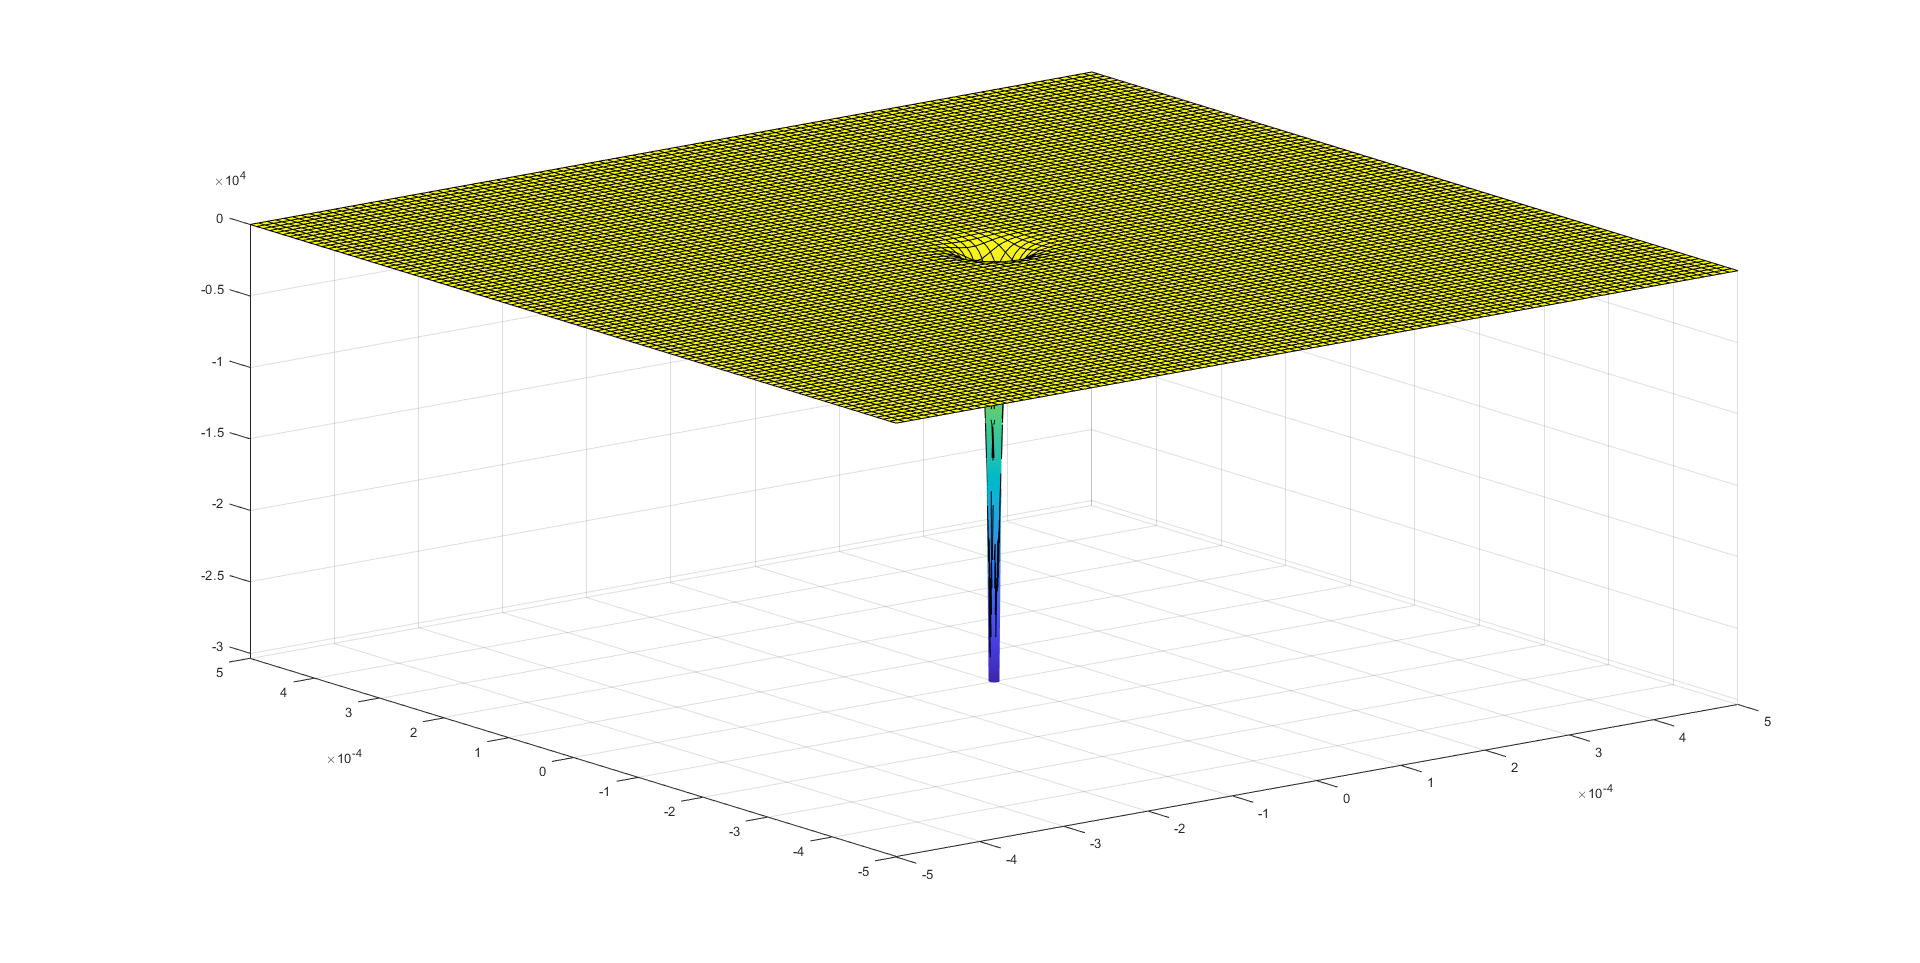
\includegraphics[scale=0.36]{spd0orig.png}
		\caption{График плотности заряда в штрихованной СО $\varphi^{\prime}$, для плоскости $z^{\prime}=0$. По осям абсцисс и ординат отложены координаты, по оси аппликат \textbf{---} плотность заряда.}
		\label{ris:rho0}
	\end{figure}
	
	\begin{figure}
		\centering
		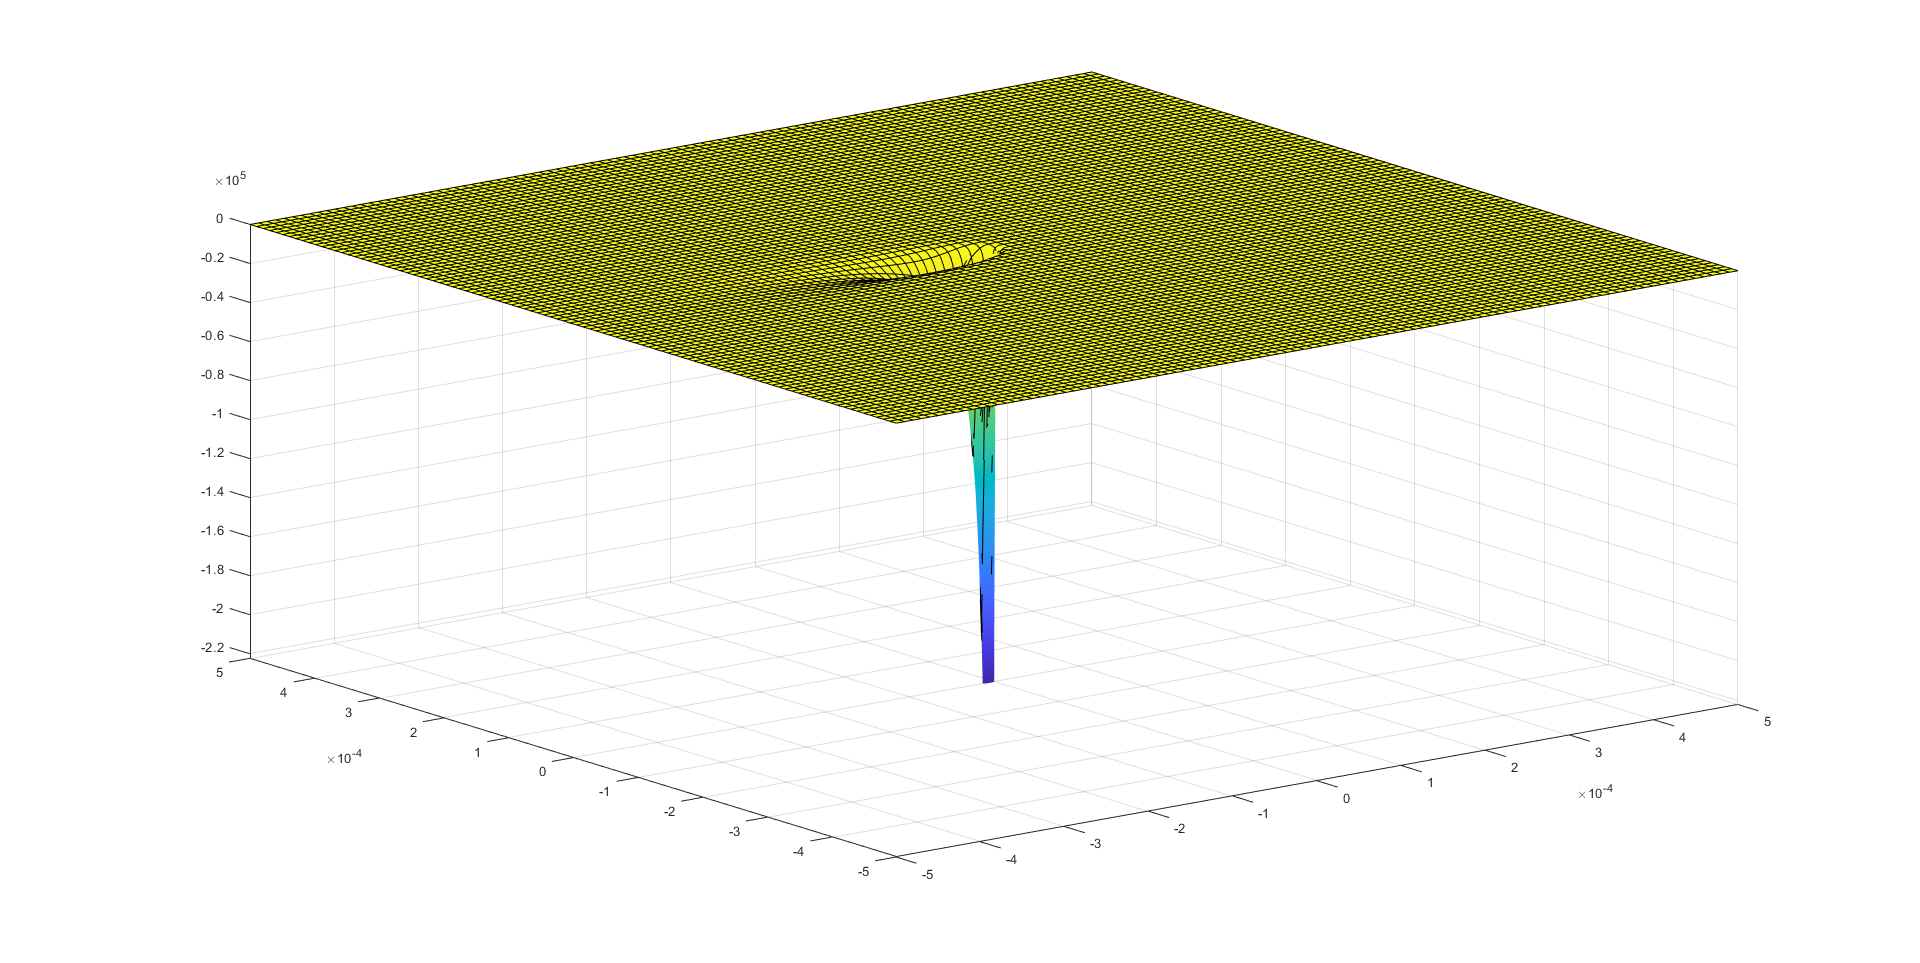
\includegraphics[scale=0.36]{spd095orig.png}
		\caption{График плотности заряда в лабораторной СО $\varphi$ при $\vec r_{0}=0$ и $\vec \beta_0 = (0.95, \ 0, \ 0)$. Остальное \textbf{---} аналогично рис. \ref{ris:rho0}}
		\label{ris:rho095}
	\end{figure}
	
	\begin{figure}
		\centering
		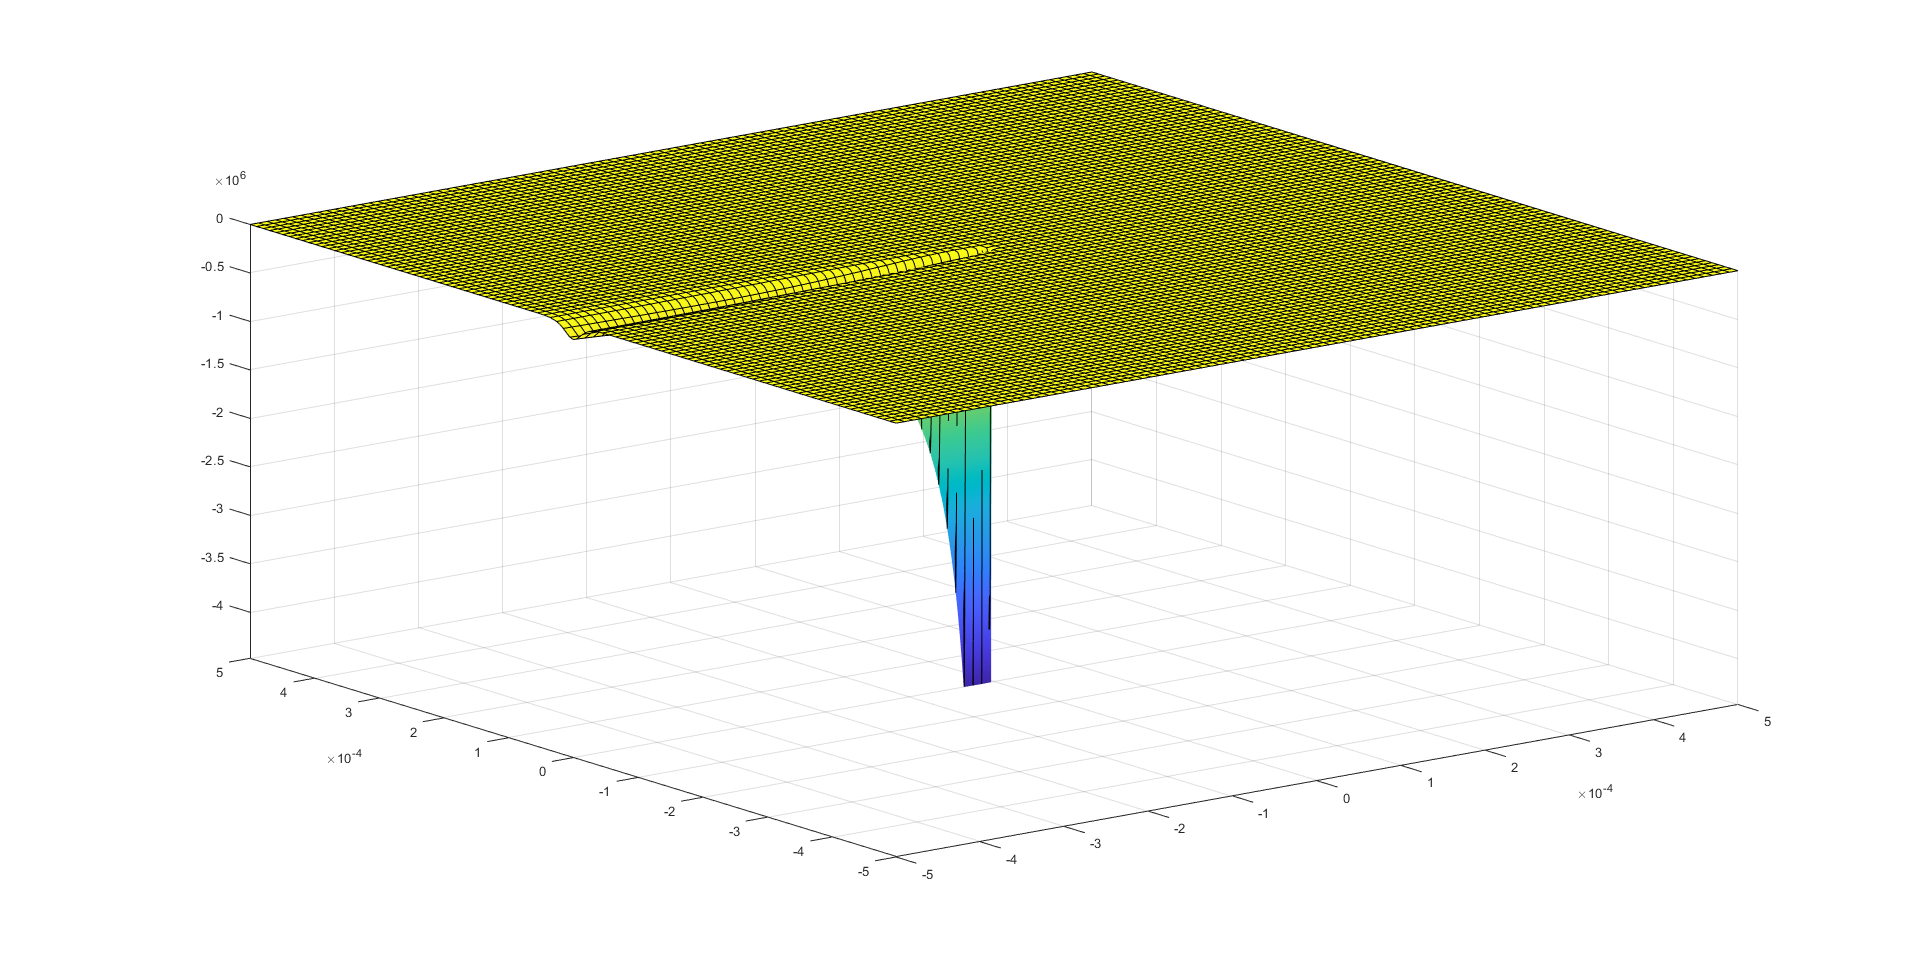
\includegraphics[scale=0.36]{spd0999orig.png}
		\caption{График плотности заряда в лабораторной СО $\varphi$ при $\vec r_{0}=0$ и $\vec \beta_0 = (0.999, \ 0, \ 0)$. Остальное \textbf{---} аналогично рис. \ref{ris:rho0}}
		\label{ris:rho0999}
	\end{figure}
	
	\begin{figure}
		\centering
		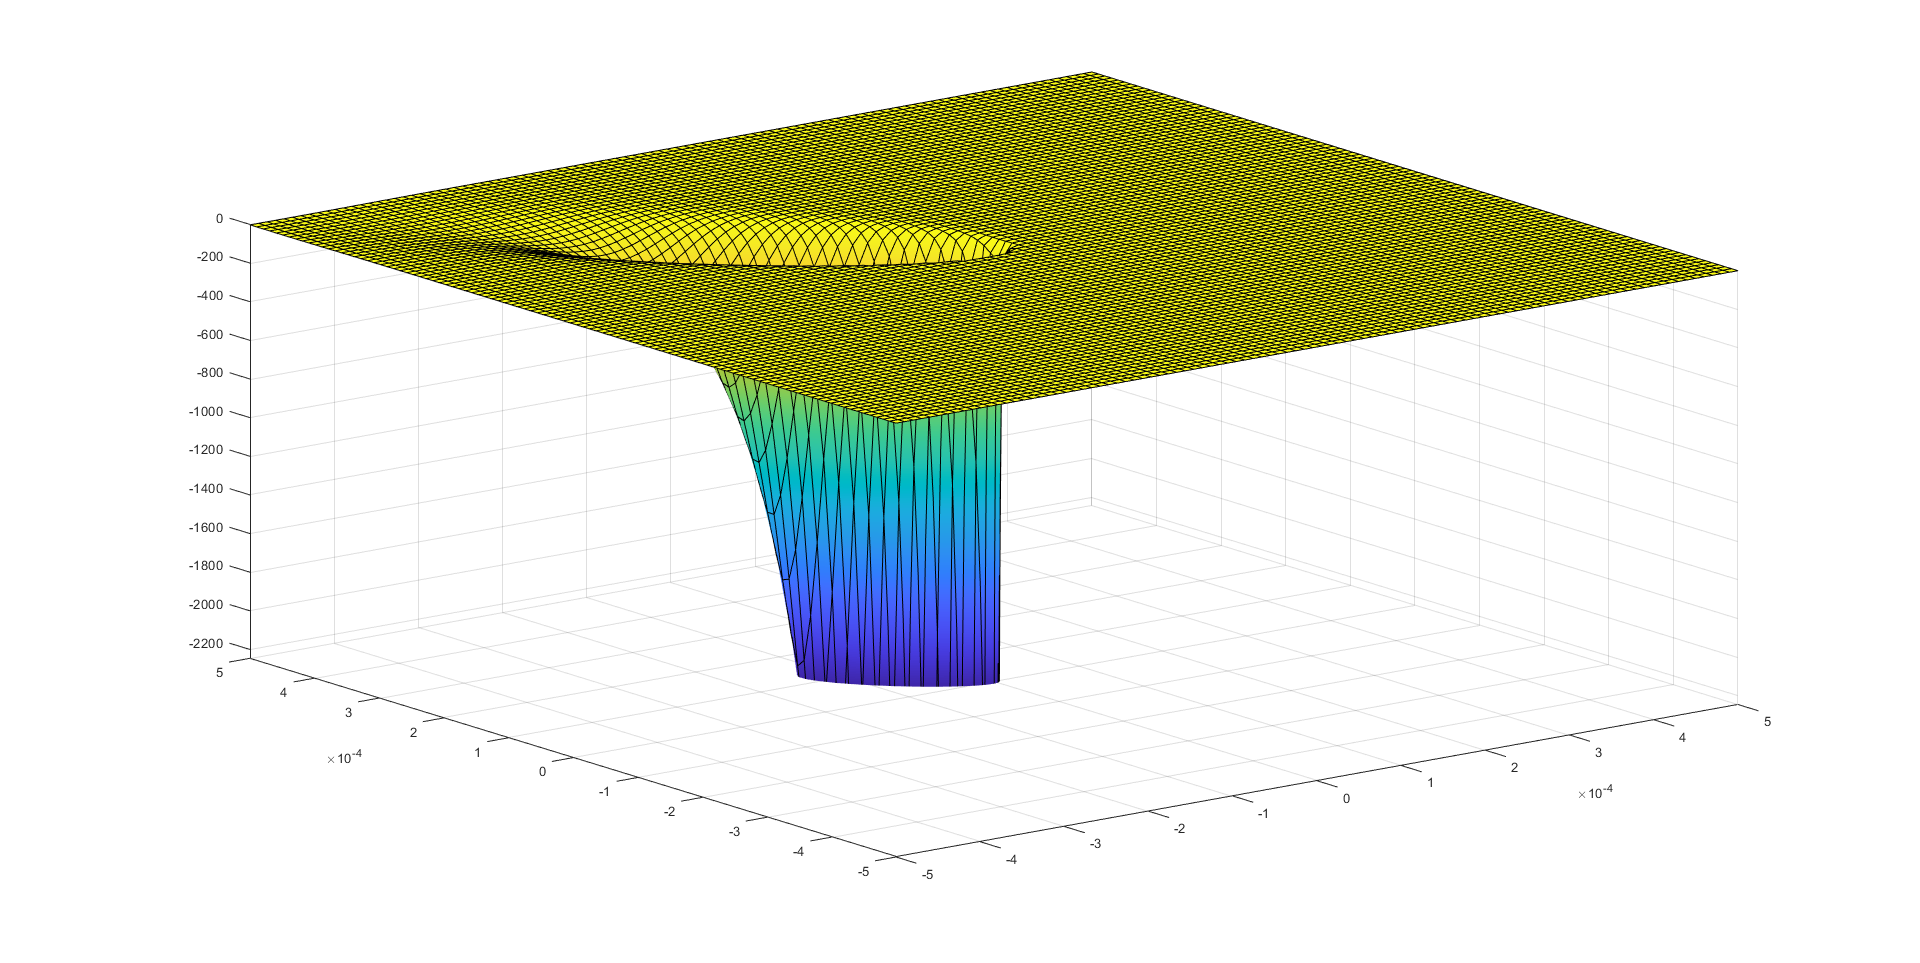
\includegraphics[scale=0.36]{diagspd095orig.png}
		\caption{График плотности заряда в лабораторной СО $\varphi$ при $\vec r_{0}=0$ и $\vec \beta_0 = (0.67, \ -0.67, \ 0)$. Остальное \textbf{---} аналогично рис. \ref{ris:rho0}}
		\label{ris:rho095diag}
	\end{figure}
	
	\newpage
	\begin{thebibliography}{0}
		\bibitem{land5} Ландау Л. Д., Лифшиц Е. М. \textit{Статистическая физика. Часть 1} \textbf{---} М., Наука, 1976.
		\bibitem{magn} Blundell S. \textit{Magnetism in Condensed Matter} \textbf{---} Oxford University Press, 2001.
		\bibitem{plasma} Котельников И. А., Ступаков Г. В. \textit{Лекции по физике плазмы: Учеб. пособие для студентов физического факультета НГУ} \textbf{---} Новосибирск, Новосиб. ун-т., 1996
		\bibitem{li-wich} Kirk T. McDonald \textit{Lienard-Wiechert Potential and Fields via Lorentz Transformations} (April 7, 1979; updated April 25, 2017) \\ \url{http://kirkmcd.princeton.edu/examples/lw_potentials.pdf}
	\end{thebibliography}
\end{document}